%; whizzy chapter
% -initex iniptex -latex platex -format platex -bibtex jbibtex -fmt fmt
% 以上 whizzytex を使用する場合の設定。

%     Tokyo Debian Meeting resources
%     Copyright (C) 2007 Junichi Uekawa

%     This program is free software; you can redistribute it and/or modify
%     it under the terms of the GNU General Public License as published by
%     the Free Software Foundation; either version 2 of the License, or
%     (at your option) any later version.

%     This program is distributed in the hope that it will be useful,
%     but WITHOUT ANY WARRANTY; without even the implied warranty of
%     MERCHANTABILITY or FITNESS FOR A PARTICULAR PURPOSE.  See the
%     GNU General Public License for more details.

%     You should have received a copy of the GNU General Public License
%     along with this program; if not, write to the Free Software
%     Foundation, Inc., 51 Franklin St, Fifth Floor, Boston, MA  02110-1301 USA

%   Pdf作成手順
% dvipdfmx debianmeetingresume200606.dvi
%  preview (shell-command (concat "evince " (replace-regexp-in-string "tex$" "pdf"(buffer-file-name)) "&"))
% 画像ファイルを処理するためにはebbを利用してboundingboxを作成。
%(shell-command "cd image200606; ebb *.png")


% progress memo: 
% 5月までマージしました。6,7月については今後のマージ対象です。
% 必要な変更点は FIXME で記録しています。


%%ここからヘッダ開始。

\documentclass[mingoth,a4paper]{jsarticle}
\usepackage[dvipdfmx]{graphicx}
\usepackage{fancybox}
\usepackage{longtable}
\usepackage{ascmac}	% 囲み (screen,itembox)
\usepackage{fancyvrb}   % 囲み Verbatim のために必要
\usepackage[dvipdfmx]{hyperref}
\usepackage{url}
\usepackage[dvipdfmx]{color}
\usepackage{wrapfig} % 図のまわりこみ
\usepackage{nextpage}
\usepackage{multicol}

% 日付を定義する、毎月変わります。
\newcommand{\debmtgyear}{2007}
\newcommand{\debmtgdate}{19}
\newcommand{\debmtgmonth}{5}
\newcommand{\debmtgnumber}{28}

%http://www.naney.org/diki/dk/hyperref.html
%日本語EUC系環境の時
\AtBeginDvi{\special{pdf:tounicode EUC-UCS2}}
%シフトJIS系環境の時
%\AtBeginDvi{\special{pdf:tounicode 90ms-RKSJ-UCS2}}

%% spacing の設定をする。外枠を減らす。
\setlength\headheight{0mm}
\setlength\topmargin{-20mm}
\setlength\headsep{0mm}
\setlength\topskip{3mm}
\setlength\maxdepth{4pt}
\setlength\columnsep{6mm}
\setlength\textheight{252mm}
\setlength\topmargin{-5mm}
\setlength\textwidth{170mm}
\setlength\oddsidemargin{-5mm}
\setlength\evensidemargin{-5mm}

% commandline環境を定義。画面入出力についてはcommandline環境
% で表記する
\newenvironment{commandline}%
{\VerbatimEnvironment
  \begin{Sbox}\begin{minipage}{15cm}\begin{fontsize}{7.3}{7.3} \begin{BVerbatim}}%
{\end{BVerbatim}\end{fontsize}\end{minipage}\end{Sbox}
  \setlength{\fboxsep}{8pt}\begin{screen}{\TheSbox}\end{screen}}


%%% start of santaku
\makeatletter
\newwrite\tf@jqz
\immediate\openout\tf@jqz\jobname.jqz\relax
\makeatother
\newcounter{santakucounter}
\newcommand{\santaku}[5]{%
\addtocounter{santakucounter}{1}

\addtocontents{jqz}{\arabic{santakucounter}. #5\\}
\begin{minipage}{1\hsize}
問題\arabic{santakucounter}. 
#1\\
□ A #2\\
□ B #3\\
□ C #4
\end{minipage}
\hspace{1cm}
\\


}
%%% end of santaku

\newcommand{\emptyspace}{(\underline{\hspace{1cm}})}

\newcommand{\subsubsubsection}[1]{%
\vspace{1zw}{\bf #1}\\}

% sectionをセンタリングする
\makeatletter
  \renewcommand{\section}{\@startsection{section}{1}{\z@}%
    {\Cvs \@plus.5\Cdp \@minus.2\Cdp}% 前アキ
    {.5\Cvs \@plus.3\Cdp}% 後アキ
    {\normalfont\Huge\headfont\raggedright\centering}} % style
\makeatother

% section の代わりの環境
\newcommand{\dancersection}[2]{%
\newpage
東京エリアDebian勉強会 \debmtgyear{}年
\hrule
\vspace{0.5mm}
\hrule
%
\vspace{4cm}
\hrule
\vspace{0.5mm}
\hrule
%
\vspace{-7cm}
\begin{minipage}[b]{0.7\hsize}
\section{#1}
\hfill{}#2\\
\vspace{2cm}
\end{minipage}
\begin{minipage}[b]{0.3\hsize}
\hfill{}
\includegraphics[height=8cm]{image200502/openlogo-nd.eps}\\
\end{minipage}
%
%\hfill{}
\includegraphics[width=16cm]{image2006-natsu/guruguru-sand-light.png}\\
\vspace{-1cm}
}

% for dancerj
\newcommand{\fgref}[1]{図\ref{#1}}
\newcommand{\tbref}[1]{表\ref{#1}}

% BTSの番号を見るためのコマンド
\newcommand{\debianbug}[1]{#1\footnote{\url{http://bugs.debian.org/#1}}}

\begin{document}

\begin{titlepage}

\includegraphics[height=252mm]{image2007-natsu/2007-summer.eps}

%\thispagestyle{empty}
\end{titlepage}

\newpage
\begin{minipage}[]{0.2\hsize}
 \definecolor{titleback}{gray}{0.9}
 \colorbox{titleback}{\rotatebox{90}{\fontsize{80}{80} {\gt デビアン勉強会} }}
\end{minipage}
\begin{minipage}[]{0.8\hsize}
\hrule
\vspace{1mm}
\hrule
\setcounter{tocdepth}{1}
{\small
 \tableofcontents}
\vspace{1mm}
\hrule
\vspace{3cm}

{
\large
\begin{itembox}{\bf『あんどきゅめんてっど でびあん』について}
本書は、東京周辺で毎月行なわれている『東京エリア Debian 勉強会』で
使用された資料・小ネタ・必殺技などを一冊にまとめたものです。
収録範囲は勉強会第23回から第28回まで。
内容は無保証、つっこみなどがあれば勉強会にて。
\end{itembox}
}
\end{minipage}




\dancersection{パッチ管理ツールquiltの使い方}{小林 儀匡}
%\label{sec:quilt}

本節ではパッチ管理ツールquilt\footnote{\url{http://savannah.nongnu.org/projects/quilt}}を取り上げ、
その基本操作を中心に説明します。
quiltはDebianに特有な (つまりDebian-specificな) ソフトウェアではなく、
Debianとは全く関係のない場所で開発されています。
しかし、このツールがDebianパッケージの作成に有用であることを理解し、
実際に作成に使用してもらえたら嬉しい限りです。

\subsection{はじめに}

\subsubsection{パッチとは}

開発者であれば当然のように作成したり読んだり当てたりしたことがある\textbf{パッチ}ですが、
一般ユーザには見慣れないものだと思います。
そこで、最初にパッチについて説明しておきます。

パッチとは、2つのファイルの差分を含むファイルのことです。
次のような2つのファイルがあるとしましょう。

\begin{commandline}
nori1[3:57]%  cat file1.txt                                        saba:~/tmp/q
あいうえお
かきくけこ
さしすせそ
たちつてと
なにぬねの
はひふへほ
まみむめも
や ゆ よ
らりるれろ
わ を ん
nori1[3:58]%  cat file2.txt                                        saba:~/tmp/q
あいうえお
ばびぶべぼ
たちつてと
なにぬねの
まみむめも
や ゆ よ
らりるれろ
わ を ん
\end{commandline}

これらのファイルのどこが違っているかすぐにわかりますか?
一々目で比べる必要はありません。
\texttt{diff}コマンドでこれらの差分をとることができます。

\begin{commandline}
nori1[3:57]%  diff file1.txt file2.txt                             saba:~/tmp/q
2,3c2
< かきくけこ
< さしすせそ
---
> ばびぶべぼ
6d4
< はひふへほ
\end{commandline}

\texttt{file1.txt}と\texttt{file2.txt}の内容や行番号を考えれば、
なんとなく意味がわかると思います。
それでかまいません。
もちろん、この出力を手で書けるようにならなくてかまいません。

この形式でもよいのですが、
通常は\texttt{diff}コマンドに\texttt{-u}オプションをつけ、
次のような\textbf{unified diff}という形式で出力させます。

\begin{commandline}
nori1[3:57]%  diff -u file1.txt file2.txt                          saba:~/tmp/q
--- file1.txt   Thu Jan 18 03:57:14 2007
+++ file2.txt   Thu Jan 18 03:57:22 2007
@@ -1,9 +1,7 @@
 あいうえお
-かきくけこ
-さしすせそ
+ばびぶべぼ
 たちつてと
 なにぬねの
-はひふへほ
 まみむめも
 や ゆ よ
 らりるれろ
\end{commandline}

こちらのほうが、
追加・削除された行がどちらのファイルに所属するのか、
そしてファイルのどのような部分が異なるのかがわかりやすいでしょう。

パッチとは要は、次のようにしてこういった出力をファイルに収めたものです。

\begin{commandline}
nori1[3:58]%  diff -u file1.txt file2.txt > file.diff              saba:~/tmp/q
\end{commandline}

ただし、全く縁のない2つのファイルであれば差分はわざわざファイルに収める必要はないでしょう。
わざわざパッチを作成するのは、
ファイルに変更を加える前後の差分を見たり、
後で紹介するように機械的な処理で変更を加えられるようにしたりするためです。
そこで、
ここまでは\texttt{file1.txt}と\texttt{file2.txt}は無縁のファイルとしてきましたが、
ここからは\texttt{file1.txt}を改変したものが\texttt{file2.txt}であると考えてください。
つまり\texttt{file1.txt}が改変前のファイルで、
\texttt{file2.txt}が改変後のファイル、
パッチ\texttt{file.diff}には\texttt{file1.txt}を\texttt{file2.txt}にするための変更が含まれている、
と考えてください。

さて、作成したパッチは、\texttt{patch}コマンドを用いて、
その中に含む変更を該当ファイルに\textbf{適用する} (\textbf{当てる}) ことができます。

\begin{commandline}
nori1[4:00]%  patch < file.diff                                    saba:~/tmp/q
patching file file1.txt
\end{commandline}

こうして\texttt{file1.txt}の内容は\texttt{file2.txt}の内容と同一になります。

\begin{commandline}
nori1[4:01]%  cat file1.txt                                        saba:~/tmp/q
あいうえお
ばびぶべぼ
たちつてと
なにぬねの
まみむめも
や ゆ よ
らりるれろ
わ を ん
nori1[4:02]%  cmp file1.txt file2.txt                              saba:~/tmp/q
\end{commandline}

また、\texttt{-R}オプションを指定して逆向きに当てることもできます。

\begin{commandline}
nori1[4:18]%  patch -R < file.diff                                 saba:~/tmp/q
patching file file1.txt
nori1[4:19]%  cat file1.txt                                        saba:~/tmp/q
あいうえお
かきくけこ
さしすせそ
たちつてと
なにぬねの
はひふへほ
まみむめも
や ゆ よ
らりるれろ
わ を ん
\end{commandline}

\texttt{file1.txt}の内容は元に戻りました。

パッチは必ずしもうまく当たらないことを忘れてはなりません。
次のように、\texttt{file1.txt}の2行目を手元で改変したとします。

\begin{commandline}
nori1[5:29]%  cat file1.txt                                        saba:~/tmp/q
あいうえお
がぎぐげご
さしすせそ
たちつてと
なにぬねの
はひふへほ
まみむめも
や ゆ よ
らりるれろ
わ を ん
\end{commandline}

これに先程のパッチを当てようとすると次のようにエラーになります。

\begin{commandline}
nori1[5:30]%  patch < file.diff                                    saba:~/tmp/q
patching file file1.txt
Hunk #1 FAILED at 1.
1 out of 1 hunk FAILED -- saving rejects to file file1.txt.rej
\end{commandline}

これは、手元で与えた変更とパッチが加えたい変更が競合しているからです。

もちろん、\texttt{file1.txt}の2行目を改変する代わりに、
次のように最終行に1行加えたとします。

\begin{commandline}
nori1[5:32]%  cat file1.txt                                        saba:~/tmp/q
あいうえお
かきくけこ
さしすせそ
たちつてと
なにぬねの
はひふへほ
まみむめも
や ゆ よ
らりるれろ
わ を ん
むふふふふ
\end{commandline}

この場合、
手元で加えた変更はパッチが含む変更とは被らないので、パッチはうまく当たります\footnote{ただしあくまで形式的にであって、意味的に適切かどうかは確認する必要があります。}。

\begin{commandline}
nori1[5:36]%  patch < file.diff                                    saba:~/tmp/q
patching file file1.txt
nori1[5:52]%  cat file1.txt                                        saba:~/tmp/q
あいうえお
ばびぶべぼ
たちつてと
なにぬねの
まみむめも
や ゆ よ
らりるれろ
わ を ん
むふふふふ
\end{commandline}

これまでは1つのファイルの変更を1つのパッチに収めてきましたが、
1つのパッチに複数のファイルの変更を収めることも可能です。
以下は、\texttt{diff}に\texttt{-r}オプションを渡して、
内容の一部が異なる2つのファイルを含む2つのディレクトリの差分をパッチとして出力させた例です。

\begin{commandline}
nori1[5:14]%  diff -ur skkdic.orig skkdic > skkdic.diff              saba:~/tmp
nori1[5:14]%  cat skkdic.diff                                        saba:~/tmp
diff -ur skkdic.orig/debian/changelog skkdic/debian/changelog
--- skkdic.orig/debian/changelog        Fri Dec 15 03:36:49 2006
+++ skkdic/debian/changelog     Mon Dec 25 17:39:10 2006
@@ -1,5 +1,7 @@
 skkdic (20061130-2~pre1) unstable; urgency=low
 
+  * debian/rules: Pass the `-k' option to dh_installchangelogs so that
+    all of ChangeLog* are installed equally.
   * debian/skkdic{,-cdb,-extra}.docs: Deleted since their settings are
     now moved into debian/rules.
 
diff -ur skkdic.orig/debian/rules skkdic/debian/rules
--- skkdic.orig/debian/rules    Fri Dec 15 03:36:49 2006
+++ skkdic/debian/rules Mon Dec 25 17:39:10 2006
@@ -2,6 +2,7 @@
 include /usr/share/cdbs/1/rules/debhelper.mk
 include /usr/share/cdbs/1/class/makefile.mk
 
+DEB_DH_INSTALLCHANGELOGS_ARGS := -k
 DEB_INSTALL_CHANGELOGS_ALL := ChangeLog
 DEB_INSTALL_DOCS_ALL := ChangeLog.* READMEs/committers.txt
 
\end{commandline}

以上で簡単なパッチの説明は終わりです。
こういったパッチは、
修正した部分を確認したり他人と修正内容をやりとりしたりするのに非常に便利で、
開発作業はこれなしではやっていけないと言っても過言ではないでしょう。
実際に使うに当たってはpatch(1)やdiff(1)のマニュアルを参照することをお勧めします。

\subsubsection{パッチ管理ツールとは}

今回説明するquiltはパッチ管理ツールです。
これは、複数のパッチを管理するためのものです。
どのような場合に必要になるのでしょう?

先程パッチとは「修正した部分を確認したり他人と修正内容をやりとりしたりするのに非常に便利」だと書きました。
その言葉に基づけば、一般にはパッチとは使い捨ての一時ファイルで短寿命です。
管理する必要はありません。

しかし、以下のようなケースを考えてみてください。
\begin{itemize}
 \item ある団体がソフトウェアfooを公開し、定期的にリリースしている。
 \item Aさんはfooを改変して使ったり再配布したりする必要がある。
 \item Aさんの改変内容には複数の論理的に異なる変更が混ざっており、fooに取り込まれるものもあれば取り込まれないものもある。
\begin{itemize}
 \item fooのバグの修正1 (小さな変更なので次のマイナーリリースで適用される。)
 \item fooのバグの修正2 (大きめの変更なので次のメジャーリリースまで適用されない。)
 \item fooのバグの修正3 (バグを回避するためのAさん独自の次善策で、開発元からのリリースでは適用されない。)
 \item :
 \item fooのバグの修正N
 \item Aさんの環境に合わせるためのMakefileの修正
\end{itemize}
\end{itemize}

Aさんが全体の変更を1つのパッチとして管理するのは不可能に近いでしょう。
fooの新しいリリースが出たときに、
元のパッチを当てても (うまく当たる部分もあるでしょうが) 間違いなくうまく当たりません。
しかも複数の変更が混ざっているのでそれを解決するのは非常に大変でしょう。

変更を複数の論理的なパッチに分割すれば、少しは管理が楽になるでしょう。
1つずつパッチを当て、うまく当たるものと当たらないものを区別できます。
当たらないもののうち、
既に開発元で加えられた修正のパッチは削除し、
残すべきなのに他の変更の影響で部分的にうまく当たらないパッチはうまく当たるよう調整します。
それらの作業は面倒かもしれませんが、
1つのパッチとして管理するのに比べれば楽でしょう。
ただし、作業中に、
現在どのパッチが当たっていてどれが当たっていないかを一々覚えておかなければならないのが大変です。

そこで登場するのがパッチ管理ツールです。
パッチ管理ツールは、複数のパッチの取り扱いを楽にするためのツールです。
具体的には、どのパッチが当たっておりどれが当たっていないかを管理できます。
また、一度に複数のパッチを当てたり外したりできるので、
全ての (あるいはある一群の) パッチがうまく当たるかどうかを概観するのも楽にできます。
Aさんがやっているような作業にはうってつけのツールです。

さて、実はDebianパッケージのメンテナ (保守担当者) はこのAさんのような作業をする必要があります。
すなわち、
開発元のリリースに複数のパッチを独自に当て、それらを管理する必要があるのです。
というのも、
一般に開発元とDebianとではリリースサイクルや品質の基準が異なるからです。
管理すべきパッチは、ソフトウェアの規模が大きくなればなるほど増えるでしょう。
そこでDebianパッケージメンテナはパッチ管理ツールを使用することが推奨されています。

ここではquiltを使用したパッチ管理を紹介します。
Debianでよく使われるパッチ管理ツールには、dpatchというものもあります。
こちらはDebianパッケージメンテナンスに特化したツールですが、
機能的にはquiltとそんなに違いはありません。
興味がある方は、2005年7月勉強会\footnote{\url{http://www.netfort.gr.jp/~dancer/column/2005-debianmeeting.html.ja\#6th}}の資料を参照してください。

\subsection{インストール}

quiltは、Debianでは\texttt{quilt}パッケージに含まれており、
\texttt{apt-get}や\texttt{aptitude}で普通にインストールできます。

\subsection{quiltの基本操作}

\subsubsection{最初に知っておくべきこと}

quiltでは一般に、\texttt{quilt <コマンド>}という書式で様々なコマンドが利用できます。
利用可能なコマンドの一覧は次のようにして参照できます。

\begin{commandline}
nori1[13:19]%  quilt --help                                             whale:~
使い方: quilt [--trace[=verbose]] [--quiltrc=XX] command [-h] ...
       quilt --version
コマンド一覧:
        add       files   import   previous  setup
        annotate  fold    mail     push      snapshot
        applied   fork    new      refresh   top
        delete    graph   next     remove    unapplied
        diff      grep    patches  rename    upgrade
        edit      header  pop      series

全コマンド共通オプション:

--trace
        コマンドをbashのトレースモード(-x)で実行。内部デバッグ用。

--quiltrc file
        ~/.quiltrc (存在しない場合は代わりに /etc/quiltrc) 以外のコン
        フィギュレーションファイルを指定。内容の詳細については PDFのド
        キュメントを参照。

--version
        バージョン情報を出力して終了。
\end{commandline}

また各コマンドのヘルプメッセージは各コマンドに\texttt{-h}オプションを指定すれば表示できます。
以下の例では\texttt{quilt add}のヘルプメッセージを表示させています。

\begin{commandline}
nori1[13:45]%  quilt add -h                                             whale:~
Usage: quilt add [-P patch] {file} ...

Add one or more files to the topmost or named patch.  Files must be
added to the patch before being modified.  Files that are modified by
patches already applied on top of the specified patch cannot be added.

-P patch
        Patch to add files to.
\end{commandline}

\subsubsection{パッチスタック}

実際にquiltを使う前に、quiltのデータ構造を知っておきましょう。
quiltは、あるツリーに対する一連のパッチを一列に並べてスタックとして管理します。

あるソースツリーに、以下のような5つのパッチを順に加えたいとします。

\begin{enumerate}
 \item r1091-remove-trailing-garbage.diff
 \item r1092-implement-distclean.diff
 \item r1094-add-readme.diff
 \item fix-ftbfs-on-m68k.diff
 \item work-around-an-error-of-libtool.diff
\end{enumerate}

このとき、
これらのパッチは\textbf{patchesディレクトリ}に含まれていなければなりません。
そして、パッチの整列順序を収めた次のような内容の\textbf{seriesファイル}\footnote{dpatchにおける\texttt{00list}と同じ役割を果たします。}がパッチディレクトリに含まれている必要があります。

\begin{screen}
\begin{verbatim}
r1091-remove-trailing-garbage.diff
r1092-implement-distclean.diff
r1094-add-readme.diff
fix-ftbfs-on-m68k.diff
work-around-an-error-of-libtool.diff
\end{verbatim}
\end{screen}

つまりまとめると、
上に挙げた5つのパッチを順に加えるようなパッチセットのデータは次のようなものです。

\begin{commandline}
nori1[14:22]%  ls patches/*             whale:~/svnwc/deb/serf/trunk/serf-0.1.0
patches/fix-ftbfs-on-m68k.diff
patches/r1091-remove-trailing-garbage.diff
patches/r1092-implement-distclean.diff
patches/r1094-add-readme.diff
patches/series
patches/work-around-an-error-of-libtool.diff
nori1[14:22]%  cat patches/series       whale:~/svnwc/deb/serf/trunk/serf-0.1.0
r1091-remove-trailing-garbage.diff
r1092-implement-distclean.diff
r1094-add-readme.diff
fix-ftbfs-on-m68k.diff
work-around-an-error-of-libtool.diff
\end{commandline}

quiltのパッチデータはこれが全てです。

なおこのデータ構造は、
\ref{subsubsec:quilt-create-patch}で後述するパッチ作成作業時にquiltが自動的に作成してくれるので、
通常は手でいじる必要はありません。
次のセクションでは、
このようなpatchesディレクトリを既にもったツリーでパッチを当てたり外したりしてみましょう。

\subsubsection{パッチスタックの操作}

さて、ではquiltを使ってみます。
まずはスタック管理のための操作を眺めてみましょう。
スタック管理に必要な操作は、もちろんpushとpopです。

最初は何もパッチが当たっていないとします。
この状態で\texttt{quilt push}を実行すると、
1番目のパッチ、つまり\texttt{r1091-remove-trailing-garbage.diff}が当たります。
このパッチは\texttt{Makefile.in}に修正を加えるものです。

\begin{commandline}
nori1[14:30]%  quilt push               whale:~/svnwc/deb/serf/trunk/serf-0.1.0
Applying patch r1091-remove-trailing-garbage.diff
patching file Makefile.in

Now at patch r1091-remove-trailing-garbage.diff
\end{commandline}

きちんと当たったようですね。
\texttt{quilt push}は、引数を与えなければ「次のパッチ」を当てるコマンドです。
これで現在ツリーは、
\texttt{r1091-remove-trailing-garbage.diff}だけが当たった状態になりました。

もう一度\texttt{quilt push}を実行します。

\begin{commandline}
nori1[15:08]%  quilt push               whale:~/svnwc/deb/serf/trunk/serf-0.1.0
Applying patch r1092-implement-distclean.diff
patching file Makefile.in

Now at patch r1092-implement-distclean.diff
\end{commandline}

次のパッチ\texttt{r1092-implement-distclean.diff}も当たりました。
これを「\texttt{r1092-implement-distclean.diff}が\textbf{一番上に来た}状態」と言うことにしましょう。
スタック (stack) とは英語で「積み重ねたもの」の意味です。
push操作ではその上にもの (quilt ではパッチ) を次々に載せていくので、
「パッチ○○まで当てられた状態」は、
言い換えれば「パッチ○○が一番上に来た状態」です。

pushの逆はpopです。
すなわち現在一番上にあるパッチを外すのは\texttt{quilt pop}です。

\begin{commandline}
nori1[15:15]%  quilt pop                whale:~/svnwc/deb/serf/trunk/serf-0.1.0
Removing patch r1092-implement-distclean.diff
Restoring Makefile.in

Now at patch r1091-remove-trailing-garbage.diff
nori1[15:15]%  quilt pop                whale:~/svnwc/deb/serf/trunk/serf-0.1.0
Removing patch r1091-remove-trailing-garbage.diff
Restoring Makefile.in

No patches applied
\end{commandline}

\texttt{quilt push}や\texttt{quilt pop}に引数としてパッチ名を与えると、
そのパッチが一番上に来た状態になるように一連のパッチを当てたり外したりします。
また引数として数値を与えると、その数だけパッチを当てたり外したりできます。
\texttt{-a}をオプションとして指定すると全てのパッチを当てたり外したりできます。

\begin{commandline}
nori1[15:17]%  quilt push 3             whale:~/svnwc/deb/serf/trunk/serf-0.1.0
Applying patch r1091-remove-trailing-garbage.diff
patching file Makefile.in

Applying patch r1092-implement-distclean.diff
patching file Makefile.in

Applying patch r1094-add-readme.diff
patching file README

Now at patch r1094-add-readme.diff
nori1[15:17]%  quilt pop r1091-remove-trailing-garbage.diff
Removing patch r1094-add-readme.diff
Removing README

Removing patch r1092-implement-distclean.diff
Restoring Makefile.in

Now at patch r1091-remove-trailing-garbage.diff
nori1[15:18]%  quilt push -a            whale:~/svnwc/deb/serf/trunk/serf-0.1.0
Applying patch r1092-implement-distclean.diff
patching file Makefile.in

Applying patch r1094-add-readme.diff
patching file README

Applying patch fix-ftbfs-on-m68k.diff
patching file Makefile.in

Applying patch work-around-an-error-of-libtool.diff
patching file Makefile.in

Now at patch work-around-an-error-of-libtool.diff
nori1[15:18]%  quilt pop -a             whale:~/svnwc/deb/serf/trunk/serf-0.1.0
Removing patch work-around-an-error-of-libtool.diff
Restoring Makefile.in

Removing patch fix-ftbfs-on-m68k.diff
Restoring Makefile.in

Removing patch r1094-add-readme.diff
Removing README

Removing patch r1092-implement-distclean.diff
Restoring Makefile.in

Removing patch r1091-remove-trailing-garbage.diff
Restoring Makefile.in

No patches applied
\end{commandline}

現在一番上にあるパッチは\texttt{quilt top}で確認できます。
現在一番上にあるパッチの次のパッチと前のパッチはそれぞれ、\texttt{quilt next}と\texttt{quilt previous}で確認できます。
現在当てられているパッチと当てられていないパッチはそれぞれ、\texttt{quilt applied}と\texttt{quilt unapplied}で確認できます。
そして、全てのパッチ、つまりseriesファイルの内容は\texttt{quilt series}で確認できます。

\begin{commandline}
nori1[15:31]%  quilt top                whale:~/svnwc/deb/serf/trunk/serf-0.1.0
No patches applied
nori1[15:31]%  quilt next               whale:~/svnwc/deb/serf/trunk/serf-0.1.0
r1091-remove-trailing-garbage.diff
nori1[15:31]%  quilt previous           whale:~/svnwc/deb/serf/trunk/serf-0.1.0
No patches applied
nori1[15:31]%  quilt applied            whale:~/svnwc/deb/serf/trunk/serf-0.1.0
No patches applied
nori1[15:31]%  quilt unapplied          whale:~/svnwc/deb/serf/trunk/serf-0.1.0
r1091-remove-trailing-garbage.diff
r1092-implement-distclean.diff
r1094-add-readme.diff
fix-ftbfs-on-m68k.diff
work-around-an-error-of-libtool.diff
nori1[15:32]%  quilt push 2             whale:~/svnwc/deb/serf/trunk/serf-0.1.0
Applying patch r1091-remove-trailing-garbage.diff
patching file Makefile.in

Applying patch r1092-implement-distclean.diff
patching file Makefile.in

Now at patch r1092-implement-distclean.diff
nori1[15:32]%  quilt top                whale:~/svnwc/deb/serf/trunk/serf-0.1.0
r1092-implement-distclean.diff
nori1[15:32]%  quilt next               whale:~/svnwc/deb/serf/trunk/serf-0.1.0
r1094-add-readme.diff
nori1[15:32]%  quilt previous           whale:~/svnwc/deb/serf/trunk/serf-0.1.0
r1091-remove-trailing-garbage.diff
nori1[15:32]%  quilt applied            whale:~/svnwc/deb/serf/trunk/serf-0.1.0
r1091-remove-trailing-garbage.diff
r1092-implement-distclean.diff
nori1[15:33]%  quilt unapplied          whale:~/svnwc/deb/serf/trunk/serf-0.1.0
r1094-add-readme.diff
fix-ftbfs-on-m68k.diff
work-around-an-error-of-libtool.diff
nori1[15:33]%  quilt series             whale:~/svnwc/deb/serf/trunk/serf-0.1.0
r1091-remove-trailing-garbage.diff
r1092-implement-distclean.diff
r1094-add-readme.diff
fix-ftbfs-on-m68k.diff
work-around-an-error-of-libtool.diff
nori1[15:33]%  quilt pop -a             whale:~/svnwc/deb/serf/trunk/serf-0.1.0
Removing patch r1092-implement-distclean.diff
Restoring Makefile.in

Removing patch r1091-remove-trailing-garbage.diff
Restoring Makefile.in

No patches applied
\end{commandline}

ある特定のファイルを変更するパッチの一覧は\texttt{quilt files}で参照可能です。
逆に、ある特定のパッチが変更するファイルの一覧は\texttt{quilt patches}で参照可能です。

\begin{commandline}
nori1[15:35]%  quilt files r1091-remove-trailing-garbage.diff
Patch r1091-remove-trailing-garbage.diff is not applied
nori1[15:35]%  quilt push r1091-remove-trailing-garbage.diff
Applying patch r1091-remove-trailing-garbage.diff
patching file Makefile.in

Now at patch r1091-remove-trailing-garbage.diff
nori1[15:35]%  quilt files              whale:~/svnwc/deb/serf/trunk/serf-0.1.0
Makefile.in
nori1[15:36]%  quilt files r1091-remove-trailing-garbage.diff
Makefile.in
nori1[15:36]%  quilt pop -a             whale:~/svnwc/deb/serf/trunk/serf-0.1.0
Removing patch r1091-remove-trailing-garbage.diff
Restoring Makefile.in

No patches applied
nori1[15:36]%  quilt patches Makefile.in
r1091-remove-trailing-garbage.diff
r1092-implement-distclean.diff
fix-ftbfs-on-m68k.diff
work-around-an-error-of-libtool.diff
\end{commandline}

これでパッチスタックの操作の説明は終わりです。
パッチを含んだpatchesディレクトリが存在していれば、
その中のパッチを自由自在に当てたり外したり、
現在当たっているパッチを調べたりできるようになりました。
しかしこれだけでは何の役にも立ちません。
次のセクションではパッチを新たに追加する方法について説明します。

\subsubsection{パッチの追加}
\label{subsubsec:quilt-create-patch}

いよいよpatchesディレクトリに新たなパッチを追加します。
quiltでは\texttt{quilt new}で新たなパッチに名前をつけて作成を開始し、
適当な変更を加えた後、\texttt{quilt refresh}でパッチとして保存します。

新たなパッチを追加する場合、
まずはパッチをスタックのどこに入れるか決めます\footnote{\ref{subsec:quilt-Debian-packaging}にパッチの並べ方に関する簡単なアドバイスがあります。}。
今回は (特に意味はありませんが) 1つ目のパッチである\texttt{r1091-remove-trailing-garbage.diff}の後に入れましょう。
パッチの名前は\texttt{love-debian.diff}とし、その内容は、
次のようなlove-debianターゲットを\texttt{Makefile.in}に加えるものにしましょう。

\begin{screen}
\begin{verbatim}
love-debian:
        echo "I love debian!!"
\end{verbatim}
\end{screen}

では作成を開始します。

\begin{commandline}
nori1[17:29]%  quilt push r1091-remove-trailing-garbage.diff
Applying patch r1091-remove-trailing-garbage.diff
patching file Makefile.in

Now at patch r1091-remove-trailing-garbage.diff
nori1[17:29]%  quilt new love-debian.diff
Patch love-debian.diff is now on top
\end{commandline}

早速\texttt{Makefile.in}を編集したいところですが、少し待ってください。
実はquiltでは、
パッチに含めるファイルは予め\texttt{quilt add}で追加しておかなければなりません。

\begin{commandline}
nori1[17:29]%  quilt add Makefile.in    whale:~/svnwc/deb/serf/trunk/serf-0.1.0
File Makefile.in added to patch love-debian.diff
\end{commandline}

その上でファイルの編集をし、その内容を\texttt{quilt diff}で確認します。

\begin{commandline}
nori1[17:35]%  vim Makefile.in          whale:~/svnwc/deb/serf/trunk/serf-0.1.0
[snip]
nori1[17:38]%  quilt diff               whale:~/svnwc/deb/serf/trunk/serf-0.1.0
Index: serf-0.1.0/Makefile.in
===================================================================
--- serf-0.1.0.orig/Makefile.in	2007-01-18 17:35:11.000000000 +0900
+++ serf-0.1.0/Makefile.in	2007-01-18 17:38:38.000000000 +0900
@@ -99,6 +99,9 @@
 		$(INSTALL) -m 644 $$i $(DESTDIR)$(includedir); \
 	done
 
+love-debian:
+	echo "I love debian!!"
+
 clean:
 	rm -f $(TARGET_LIB) $(OBJECTS) $(OBJECTS:.lo=.o) $(PROGRAMS) $(TEST_OBJECTS) $(TEST_OBJECTS:.lo=.o)
 
\end{commandline}

最後に\texttt{quilt refresh}で保存します。

\begin{commandline}
nori1[17:39]%  quilt refresh            whale:~/svnwc/deb/serf/trunk/serf-0.1.0
Refreshed patch love-debian.diff
\end{commandline}

さて、実は\texttt{love-debian.diff}は1番目のパッチの後に挿入しました。
ということは、残りのパッチがうまく当たるか確認しておかなければなりません。

\begin{commandline}
nori1[17:40]%  quilt push -a            whale:~/svnwc/deb/serf/trunk/serf-0.1.0
Applying patch r1092-implement-distclean.diff
patching file Makefile.in
Hunk \#1 succeeded at 104 (offset 3 lines).

Applying patch r1094-add-readme.diff
patching file README

Applying patch fix-ftbfs-on-m68k.diff
patching file Makefile.in

Applying patch work-around-an-error-of-libtool.diff
patching file Makefile.in

Now at patch work-around-an-error-of-libtool.diff
\end{commandline}

新たな行を挿入したので「\texttt{Hunk \#1 succeeded at 104 (offset 3 lines).}」というメッセージが出ましたが、
問題なく当たりました。

\texttt{quilt series}を実行すると、
きちんと\texttt{love-debian.diff}が適切な位置に挿入されていることがわかります。

\begin{commandline}
nori1[17:41]%  quilt series             whale:~/svnwc/deb/serf/trunk/serf-0.1.0
r1091-remove-trailing-garbage.diff
love-debian.diff
r1092-implement-distclean.diff
r1094-add-readme.diff
fix-ftbfs-on-m68k.diff
work-around-an-error-of-libtool.diff
nori1[17:41]%  quilt pop -a             whale:~/svnwc/deb/serf/trunk/serf-0.1.0
Removing patch work-around-an-error-of-libtool.diff
Restoring Makefile.in

Removing patch fix-ftbfs-on-m68k.diff
Restoring Makefile.in

Removing patch r1094-add-readme.diff
Removing README

Removing patch r1092-implement-distclean.diff
Restoring Makefile.in

Removing patch love-debian.diff
Restoring Makefile.in

Removing patch r1091-remove-trailing-garbage.diff
Restoring Makefile.in

No patches applied
\end{commandline}

さて、パッチを作成した後になって気付いたのですが、
love-debianターゲットが表示する文字列の中の「debian」は「Debian」と大文字にした方がよさそうです。
このようなときはパッチを改変しましょう。
\texttt{quilt push}ないし\texttt{quilt pop}で目的のパッチ (\texttt{love-debian.diff}) を一番上に持ってきて、
エディタで\texttt{Makefile.in}に変更を施した上で\texttt{quilt refresh}で保存すればOKです。
\texttt{Makefile.in}は既にパッチ\texttt{love-debian.diff}の変更対象に含まれているので、
エディタでの編集前に\texttt{quilt add}で追加する必要はありません。

\begin{commandline}
nori1[17:54]%  quilt push love-debian.diff
Applying patch r1091-remove-trailing-garbage.diff
patching file Makefile.in

Applying patch love-debian.diff
patching file Makefile.in

Now at patch love-debian.diff
nori1[17:59]%  vim Makefile.in          whale:~/svnwc/deb/serf/trunk/serf-0.1.0
[snip]
nori1[18:01]%  quilt diff               whale:~/svnwc/deb/serf/trunk/serf-0.1.0
Index: serf-0.1.0/Makefile.in
===================================================================
--- serf-0.1.0.orig/Makefile.in	2007-01-18 17:38:38.000000000 +0900
+++ serf-0.1.0/Makefile.in	2007-01-18 18:01:35.000000000 +0900
@@ -99,6 +99,9 @@
 		$(INSTALL) -m 644 $$i $(DESTDIR)$(includedir); \
 	done
 
+love-debian:
+	echo "I love Debian!!"
+
 clean:
 	rm -f $(TARGET_LIB) $(OBJECTS) $(OBJECTS:.lo=.o) $(PROGRAMS) $(TEST_OBJECTS) $(TEST_OBJECTS:.lo=.o)
 
nori1[18:01]%  quilt refresh            whale:~/svnwc/deb/serf/trunk/serf-0.1.0
Refreshed patch love-debian.diff
\end{commandline}

さて、このパッチを眺めているうちにまた気が変わって、
\texttt{design-guide.txt}という別のファイルにも変更を加え、
このパッチに含めようと思い立ちました。
\texttt{design-guide.txt}は今のところ\texttt{love-debian.diff}の変更対象外なので、
今度は、
編集する前に\texttt{quilt add}で変更対象に追加しておかなければなりません。
\texttt{quilt add design-guide.txt}を実行した上でエディタで\texttt{design-guide.txt}を開いてもよいのですが、
面倒なのでここでは\texttt{quilt edit}コマンドを実行しましょう。
このコマンドは、
「引数のファイルを\texttt{quilt add}で追加した上で、
環境変数\texttt{EDITOR}で指定されたエディタでそのファイルを開く」という、
2つの操作をまとめて実行するためのものです。

\begin{commandline}
nori1[18:19]%  quilt edit design-guide.txt
[snip]
nori1[18:21]%  quilt diff               whale:~/svnwc/deb/serf/trunk/serf-0.1.0
Index: serf-0.1.0/Makefile.in
===================================================================
--- serf-0.1.0.orig/Makefile.in	2007-01-18 17:55:20.000000000 +0900
+++ serf-0.1.0/Makefile.in	2007-01-18 18:01:35.000000000 +0900
@@ -99,6 +99,9 @@
 		$(INSTALL) -m 644 $$i $(DESTDIR)$(includedir); \
 	done
 
+love-debian:
+	echo "I love Debian!!"
+
 clean:
 	rm -f $(TARGET_LIB) $(OBJECTS) $(OBJECTS:.lo=.o) $(PROGRAMS) $(TEST_OBJECTS) $(TEST_OBJECTS:.lo=.o)
 
Index: serf-0.1.0/design-guide.txt
===================================================================
--- serf-0.1.0.orig/design-guide.txt	2007-01-18 18:19:30.000000000 +0900
+++ serf-0.1.0/design-guide.txt	2007-01-18 18:20:40.000000000 +0900
@@ -9,6 +9,7 @@
   4. Bucket Read Functions
   5. Versioning
   6. Bucket lifetimes
+  7. Love Debian
 
 
 -----------------------------------------------------------------------------
@@ -150,3 +151,10 @@
 
 
 -----------------------------------------------------------------------------
+
+7. LOVE DEBIAN
+
+Hey, please love Debian.
+
+
+-----------------------------------------------------------------------------
nori1[18:22]%  quilt refresh            whale:~/svnwc/deb/serf/trunk/serf-0.1.0
Refreshed patch love-debian.diff
\end{commandline}

これで新たなパッチ\texttt{love-debian.diff}の内容は完成です。
しかしこれだけだと後で何をしたいパッチだかわからなくなりそうです。
最後に、パッチの説明を加えておきましょう。
quiltでは、
パッチの内容を説明するヘッダを操作するコマンドは\texttt{quilt header}です。
\texttt{-e}オプションを指定してコマンドを実行すると、
環境変数\texttt{EDITOR}のエディタでパッチのヘッダを編集できます。
また、何もオプションを与えずに実行するとヘッダを表示できます。

\begin{commandline}
nori1[18:37]%  quilt header             whale:~/svnwc/deb/serf/trunk/serf-0.1.0
nori1[18:37]%  quilt header -e          whale:~/svnwc/deb/serf/trunk/serf-0.1.0
[snip]
nori1[18:41]%  quilt header             whale:~/svnwc/deb/serf/trunk/serf-0.1.0
A patch to show my love for Debian.
\end{commandline}

本セクションでは、
新たにパッチを作成する手順を学びました。
これで自由にパッチを追加・編集できます。
次のセクションでは、
開発元が加えた変更への対応方法を学びます。

\subsubsection{開発元が加えた変更への対応}

パッチをいじれるようになったところで、
開発元が新しいリリースなどで加えた変更に対応してみましょう。
この作業では、\texttt{quilt push}の\texttt{-f}オプションが役立ちます。

開発元が加えた変更をマージする前に、まずやっておかなければならないことがあります。
それは、ツリーにパッチが適用されていない状態にすることです。
既に説明したように、
適用されているパッチを全て外すには\texttt{quilt pop -a}を実行します。

\begin{commandline}
nori1[20:00]%  quilt pop -a             whale:~/svnwc/deb/serf/trunk/serf-0.1.0
Removing patch love-debian.diff
Restoring Makefile.in
Restoring design-guide.txt

Removing patch r1091-remove-trailing-garbage.diff
Restoring Makefile.in

No patches applied
\end{commandline}

その上で、ツリーのファイルを、開発元が新しくリリースしたものに差し替えます (つまり開発元が加えた変更をマージします)。
ここでは以下のような変更が入ったとします。

\begin{itemize}
 \item \texttt{Makefile.in}へのloveターゲットとclean-loveターゲットの追加 (\texttt{love-debian.diff}が変更する部分と同じ部分を改変するので、競合)
 \item \texttt{README}ファイルの追加 (\texttt{r1094-add-readme.diff}の修正内容そのもの)
\end{itemize}

さあ、新しいツリーにパッチを当てようとするとどうなるでしょうか。
とりあえず\texttt{quilt push -a}で一度に全て当てようとしてみましょう。

\begin{commandline}
nori1[20:32]%  quilt push -a            whale:~/svnwc/deb/serf/trunk/serf-0.1.0
Applying patch r1091-remove-trailing-garbage.diff
patching file Makefile.in
Hunk #1 succeeded at 103 with fuzz 2 (offset 3 lines).

Applying patch love-debian.diff
patching file Makefile.in
Hunk #1 FAILED at 99.
1 out of 1 hunk FAILED -- rejects in file Makefile.in
patching file design-guide.txt
Patch love-debian.diff does not apply (enforce with -f)
nori1[20:32]%  quilt top                whale:~/svnwc/deb/serf/trunk/serf-0.1.0
r1091-remove-trailing-garbage.diff
\end{commandline}

\texttt{love-debian.diff}を当てるのに失敗して、
そこでパッチの適用が止まってしまいました。
そこで、\texttt{-f}オプションを\texttt{quilt push}につけて、
\texttt{love-debian.diff}を強制的に適用してみます。

\begin{commandline}
nori1[20:33]%  quilt push -f            whale:~/svnwc/deb/serf/trunk/serf-0.1.0
Applying patch love-debian.diff
patching file Makefile.in
Hunk #1 FAILED at 99.
1 out of 1 hunk FAILED -- saving rejects to file Makefile.in.rej
patching file design-guide.txt
Applied patch love-debian.diff (forced; needs refresh)
\end{commandline}

\texttt{Makefile.in}がどうなったか眺めてみると、
先程love-debianターゲットを加えた箇所に、
次のようにloveターゲットとclean-loveターゲットが追加されています。

\begin{commandline}
nori1[20:37]%  cat Makefile.in          whale:~/svnwc/deb/serf/trunk/serf-0.1.0
[snip]
		$(INSTALL) -m 644 $$i $(DESTDIR)$(includedir); \
	done
love:
	echo "Making love..."
clean-love:
	echo "Clearing my old love..."
clean:
	rm -f $(TARGET_LIB) $(OBJECTS) $(OBJECTS:.lo=.o) $(PROGRAMS) $(TEST_OBJECTS) $(TEST_OBJECTS:.lo=.o)
[snip]
\end{commandline}

\texttt{quilt push -f}からのメッセージにあるように、
パッチ適用の拒否の理由は\texttt{Makefile.in.rej}に記されています。
念のため覗いてみましょう。

\begin{commandline}
***************
*** 99,104 ****
  		$(INSTALL) -m 644 $$i $(DESTDIR)$(includedir); \
  	done
  
  clean:
  	rm -f $(TARGET_LIB) $(OBJECTS) $(OBJECTS:.lo=.o) $(PROGRAMS) $(TEST_OBJECTS) $(TEST_OBJECTS:.lo=.o)
  
--- 99,107 ----
  		$(INSTALL) -m 644 $$i $(DESTDIR)$(includedir); \
  	done
  
+ love-debian:
+ 	echo "I love Debian!!"
+ 
  clean:
  	rm -f $(TARGET_LIB) $(OBJECTS) $(OBJECTS:.lo=.o) $(PROGRAMS) $(TEST_OBJECTS) $(TEST_OBJECTS:.lo=.o)
  
\end{commandline}

これは\textbf{context diff}と呼ばれる形式ですが、意味が掴めればかまいません。
上で説明したように、
love-debianターゲットを加えるための、cleanターゲットの前の3行がうまく当たらなかったことがわかるでしょう。

強制的にパッチを適用した結果がどうなったかわかったところで、
削除されてしまった大切なlove-debianターゲットを\texttt{Makefile.in}に再度追加した上で、
\texttt{quilt push -f}からのメッセージにあるようにパッチを更新 (refresh) しましょう。

\begin{commandline}
nori1[20:45]%  vim Makefile.in          whale:~/svnwc/deb/serf/trunk/serf-0.1.0
[snip]
nori1[20:54]%  quilt diff               whale:~/svnwc/deb/serf/trunk/serf-0.1.0
Index: serf-0.1.0/Makefile.in
===================================================================
--- serf-0.1.0.orig/Makefile.in	2007-01-18 20:32:13.000000000 +0900
+++ serf-0.1.0/Makefile.in	2007-01-18 20:52:22.000000000 +0900
@@ -102,6 +102,10 @@
 	echo "Making love..."
 clean-love:
 	echo "Clearing my old love..."
+
+love-debian:
+	echo "I love Debian!!"
+
 clean:
 	rm -f $(TARGET_LIB) $(OBJECTS) $(OBJECTS:.lo=.o) $(PROGRAMS) $(TEST_OBJECTS) $(TEST_OBJECTS:.lo=.o)
 
Index: serf-0.1.0/design-guide.txt
===================================================================
--- serf-0.1.0.orig/design-guide.txt	2007-01-18 20:31:56.000000000 +0900
+++ serf-0.1.0/design-guide.txt	2007-01-18 20:36:10.000000000 +0900
@@ -9,6 +9,7 @@
   4. Bucket Read Functions
   5. Versioning
   6. Bucket lifetimes
+  7. Love Debian
 
 
 -----------------------------------------------------------------------------
@@ -150,3 +151,10 @@
 
 
 -----------------------------------------------------------------------------
+
+7. LOVE DEBIAN
+
+Hey, please love Debian.
+
+
+-----------------------------------------------------------------------------
nori1[20:54]%  quilt refresh            whale:~/svnwc/deb/serf/trunk/serf-0.1.0
Refreshed patch love-debian.diff
\end{commandline}

さあ、これで\texttt{love-debian.diff}の問題は解決しました。
再び\texttt{quilt push -a}で残りのパッチを全て当てようとしてみましょう。

\begin{commandline}
nori1[20:55]%  quilt push -a            whale:~/svnwc/deb/serf/trunk/serf-0.1.0
Applying patch r1092-implement-distclean.diff
patching file Makefile.in
Hunk #1 succeeded at 108 (offset 7 lines).

Applying patch r1094-add-readme.diff
The next patch would create the file README,
which already exists!  Applying it anyway.
patching file README
Patch attempted to create file README, which already exists.
Hunk #1 FAILED at 1.
1 out of 1 hunk FAILED -- rejects in file README
Patch r1094-add-readme.diff can be reverse-applied
\end{commandline}

今度は\texttt{r1094-add-readme.diff}を当てるのに失敗して、
そこでパッチの適用が止まってしまいました。
メッセージによれば、このパッチは逆に当てることができます。
それはすなわち、このパッチが既に当たった状態であることを意味します。
開発元で\texttt{README}を追加してくれたので、
\texttt{README}を追加するための\texttt{r1094-add-readme.diff}は不要になったのでした。
そこで、このパッチは削除することにします。

\begin{commandline}
nori1[21:05]%  quilt delete r1094-add-readme.diff
Removed patch r1094-add-readme.diff
\end{commandline}

これで\texttt{r1094-add-readme.diff}の問題も解決です。
再び\texttt{quilt push -a}で残りのパッチを全て当てようとしてみましょう。

\begin{commandline}
nori1[21:05]%  quilt push -a            whale:~/svnwc/deb/serf/trunk/serf-0.1.0
Applying patch fix-ftbfs-on-m68k.diff
patching file Makefile.in

Applying patch work-around-an-error-of-libtool.diff
patching file Makefile.in

Now at patch work-around-an-error-of-libtool.diff
\end{commandline}

全てうまく当たりました。
これで一連のパッチはうまく当たるようになりました。

\begin{commandline}
nori1[21:06]%  quilt pop -a             whale:~/svnwc/deb/serf/trunk/serf-0.1.0
Removing patch work-around-an-error-of-libtool.diff
Restoring Makefile.in

Removing patch fix-ftbfs-on-m68k.diff
Restoring Makefile.in

Removing patch r1092-implement-distclean.diff
Restoring Makefile.in

Removing patch love-debian.diff
Restoring Makefile.in
Restoring design-guide.txt

Removing patch r1091-remove-trailing-garbage.diff
Restoring Makefile.in

No patches applied
\end{commandline}

\subsubsection{パッチの依存関係の可視化}

quiltの\texttt{quilt graph}コマンドとGraphvizを使うと、
適用されたパッチの依存関係を可視化できます。

最初に、全てのパッチを当てておきます。

\begin{commandline}
nori1[22:18]%  quilt push -a            whale:~/svnwc/deb/serf/trunk/serf-0.1.0
Applying patch r1091-remove-trailing-garbage.diff
patching file Makefile.in
Hunk #1 succeeded at 103 with fuzz 2 (offset 3 lines).

Applying patch love-debian.diff
patching file Makefile.in
patching file design-guide.txt

Applying patch r1092-implement-distclean.diff
patching file Makefile.in
Hunk #1 succeeded at 108 (offset 7 lines).

Applying patch fix-ftbfs-on-m68k.diff
patching file Makefile.in

Applying patch work-around-an-error-of-libtool.diff
patching file Makefile.in

Now at patch work-around-an-error-of-libtool.diff
\end{commandline}

この状態で何も与えずに\texttt{quilt graph}を実行すると、
Graphviz用のソースファイルが出力されます。
これは、同じファイルを変更する複数のパッチの間に依存関係がある、
として計算した結果です。

\begin{commandline}
nori1[22:18]%  quilt graph              whale:~/svnwc/deb/serf/trunk/serf-0.1.0
digraph dependencies {
        n0 [label="r1091-remove-trailing-garbage.diff"];
        n1 [label="love-debian.diff"];
        n2 [label="r1092-implement-distclean.diff"];
        n3 [label="fix-ftbfs-on-m68k.diff"];
        n4 [style=bold,label="work-around-an-error-of-libtool.diff"];
        n0 -> n1 [len="1.39"];
        n1 -> n2 [len="1.39"];
        n2 -> n3 [len="1.39"];
        n3 -> n4 [len="1.39"];
}
\end{commandline}

このソースを例えば\texttt{graph.dot}というファイルに保存すると、
Graphvizを使って (例えば\texttt{dot -Tpng graph.dot -o graph.png}などと実行して) 様々な形式のファイルが生成できます。
しかし、psを出力するのであれば次のように直接出力するのが楽でしょう。

\begin{commandline}
nori1[22:35]%  quilt graph -T ps > patchdep-1.eps
\end{commandline}

なお、依存関係の指定はありませんが、
内部的に (\texttt{/usr/share/quilt/graph}で) Graphvizの\texttt{dot}コマンドを呼び出しているので、
実行には\texttt{graphviz}パッケージがインストールされている必要があります (\debianbug{407469})。

生成された図は図\ref{fig:patchdep-file}のようになります。

\begin{figure}[htbp]
  \begin{center}
   \includegraphics[scale=0.8]{image200701/patchdep-1.eps}
  \end{center}
  \caption{同じファイルを変更する複数のパッチの間に依存関係がある、として計算した依存関係}
  \label{fig:patchdep-file}
\end{figure}

他方で、
同じファイルを変更するだけでなくその変更領域が被っている場合に依存関係がある、
として計算すると次のようになります。
変更領域の被りが1行の場合 (図\ref{fig:patchdep-overlap-1line}) と2行 (図\ref{fig:patchdep-overlap-2line}) の場合です。

\begin{commandline}
nori1[22:44]%  quilt graph --lines=1 -T ps > patchdep-2.eps
nori1[22:44]%  quilt graph --lines=2 -T ps > patchdep-3.eps
\end{commandline}

\begin{figure}[htbp]
  \begin{center}
   \includegraphics[scale=0.8]{image200701/patchdep-2.eps}
  \end{center}
  \caption{変更領域が1行被っている場合に依存関係がある、として計算した依存関係}
  \label{fig:patchdep-overlap-1line}
\end{figure}

\begin{figure}[htbp]
  \begin{center}
   \includegraphics[scale=0.8]{image200701/patchdep-3.eps}
  \end{center}
  \caption{変更領域が2行被っている場合に依存関係がある、として計算した依存関係}
  \label{fig:patchdep-overlap-2line}
\end{figure}

\subsubsection{環境変数}
\label{subsubsec:quilt-env}

quiltでは以下のような環境変数を指定できます。
ここでは省略していますが、他にもdiff関連の環境変数がいくつかあります。

\begin{description}
 \item[\texttt{QUILT\_PATCHES}] patchesディレクトリを指定します。指定されていない場合は\texttt{patches}がパッチファイル (およびseriesファイル) の格納に使用されます。
 \item[\texttt{QUILT\_PC}] .pcディレクトリを指定します。.pcディレクトリは、どのパッチが当てられたかを管理するためのもので、指定されていない場合は\texttt{.pc}となります。
\end{description}

\subsection{Debianパッケージ作成時のquiltの使用}
\label{subsec:quilt-Debian-packaging}

Debianパッケージ作成時のパッチの管理にquiltを使用するときは、
以下を参考にしてください。

\begin{itemize}
 \item quiltはデフォルトではパッチファイルをpatchesディレクトリに入れます。しかし、Debianパッケージ作成用のパッチは、パッケージ作成に用いる他のファイルと同様\texttt{debian}ディレクトリの下にまとめて入れておくことが推奨されています。\ref{subsubsec:quilt-env}で説明した環境変数\texttt{QUILT\_PATCHES}に\texttt{debian/patches}を設定しておくとよいでしょう。
 \item cdbsではquiltをパッチ管理に使用するのに便利なルールが用意されています。使用する場合は\texttt{debian/rules}内で\texttt{/usr/share/cdbs/1/rules/patchsys-quilt.mk}をincludeしてください。なお、cdbsのこのクラスは\texttt{patches}に\texttt{debian/patches}へのsymlinkを作成します。
 \item やや一般的な話ですが、パッチを並べる順序は開発元に近い順にするとよいでしょう。つまり、開発元に既に取り込まれている変更が最初に適用され、開発元には取り込まれることのないDebian独自の変更は最後に適用されるようにすることをお勧めします。
\end{itemize}

\dancersection{dpatch についての小ネタ}{上川 純一}
\label{sec:dpatch2007}

\texttt{dpatch} を \texttt{subversion}などといっしょに使うときにもしかす
ると便利かもしれない小ネタについて御紹介します。

\subsection{インストールのしかた}

まず最初にインストールのしかたですが、
Debianシステムであれば、

\begin{commandline}
 apt-get install dpatch
\end{commandline}

でインストールできます。そうでない場合のインストールについては想定外です。

\subsection{作業のしかた}

\texttt{debian/rules} を適切に変更したあと、
\texttt{dpatch-edit-patch} で編集します。
\footnote{\texttt{/usr/share/doc/dpatch/examples/rules/rules.dh.gz}参照}

パッチは \texttt{debian/patches} 以下で管理されます。
\texttt{debian/patches/00list} ファイルに適用するパッチの一覧があり、それを参照し
て パッチを適用します。

\subsection{dpatch に含まれる各種ツールの紹介}

各種ツールがあるので何をするものなのか、見てみましょう。

\begin{description}
 \item[dpatch] メインのツールです。表立って直接利用することはありません。
	    debian/rules などから呼び出されます。
 \item[dpatch-list-patch] パッチの一覧を出力します。
 \item[dpatch-edit-patch] 編集のツールです。パッチを作成、もしくは編集する際に利用しま
	    す。\texttt{dpatch-edit-patch パッチ名 適用するパッチ} とい
	    う形で指定すると、指定した適用するパッチまでが適用された状態
	    のソースツリーが一時ディレクトリに展開された状態でシェルが起
	    動します。そこで編集し、シェルを終了 ( ctrl-D もしくは exit
	    )するとパッチが作成され、debian/patches 以下にファイルが生成されます。
 \item[dpatch-convert-diffgz] .diff.gz から dpatch ファイルを生成するた
	    めのツールです。
 \item[dpatch-get-origtargz] dpatch-edit-patch が内部的に利用するツール。
\end{description}

\subsection{debian/ディレクトリのみを展開したパッケージのメンテナンスを
  する}

dpatch で管理すると、Debianのソースパッケージのうち、
debian/以下のディレクトリに対しての変更しか発生しなくなります。
.orig.tar.gz を展開した状態でのパッケージのメンテナンスは実は必要なく、
debian/ 以下だけをバージョン管理ツールで管理して、orig.tar.gzは必要に応
じてアップストリームからダウンロードしてくるというスタイルで開発をするこ
とができます。

dpatch-get-origtargz はそのためのツールで、現在の debian/ ディレクトリに
対応した .orig.tar.gz を環境変数 \verb!DPGO_ORIGTARDIR! で指定したパス上に存在
する .orig.tar.gz から探してきます。ローカルで見付からない場合には uscan や apt-get
source などを活用して、ネットワークからダウンロードしてきてくれます。


\begin{commandline}
[12:13:55]dancer64:ecatest> ls -l
合計 0
drwxr-xr-x 5 dancer dancer 700 2007-02-17 12:09 debian
[12:12:59]dancer64:ecatest> dpatch-edit-patch -b 12_users_guide.dpatch
dpatch-edit-patch: * /tmp/ecatest/debian/patches/12_users_guide.dpatch exists, this patch will be updated.
dpatch-edit-patch: * debian/-only layout selected
パッケージリストを読み込んでいます... 完了
依存関係ツリーを作成しています... 完了
1129kB のソースアーカイブを取得する必要があります。
取得:1 http://glantank sid/main ecasound2.2 2.4.4-6 (tar) [1129kB]
1129kB を 0s で取得しました (13.2MB/s)
dpatch-edit-patch: * unpacking ecasound2.2_2.4.4.orig.tar.gz
dpatch-edit-patch: * Copying /tmp/ecatest to reference directory.
dpatch-edit-patch: * Cleaning /tmp/dpep-ref.Nn8155/ecatest
dpatch  deapply-all
12_users_guide not applied to ./ .
11_configure_in_alsa_fix not applied to ./ .
07_configure_in_maintainer_mode not applied to ./ .
rm -rf patch-stamp patch-stampT debian/patched
dh_testdir
dh_testroot
rm -f build-stamp configure-stamp
# Add here commands to clean up after the build process.

[中略]
12_users_guide not applied to ./ .
11_configure_in_alsa_fix not applied to ./ .
07_configure_in_maintainer_mode not applied to ./ .
dpatch-edit-patch: * Applying patches
applying patch 07_configure_in_maintainer_mode to ./ ... ok.
applying patch 11_configure_in_alsa_fix to ./ ... ok.
dpatch-edit-patch: * Copying reference directory /tmp/dpep-ref.Nn8155/ecatest to work directory.
dpatch-edit-patch: * Applying current 12_users_guide.dpatch for editing.
applying patch 12_users_guide to ./ ... ok.

dpatch-edit-patch:

Now launching an interactive shell in your work directory. Edit your files.
When you are done, exit the shell. When you exit the shell, your patch will be
automatically updated based on the changes in your work directory.

If you wish to abort the process, exit the shell such that it returns an exit
code of "230". This is typically done by exiting the shell with the command
'exit 230'.
[12:13:09]dancer64:ecatest>
 
\end{commandline}


\subsection{svn-buildpackage との連携}

svn-buildpackage と dpatch の連携については特に考慮されているわけではあ
りません。ただ、連携して利用できないわけではありません。利用するには下記
の点を設定すればよいでしょう。

svn-buildpackage も、 debian/ ディレクトリのみを別管理にする方法をサポー
トしています。それを利用する際に注意する点として、 orig.tar.gz の場所を
指示するために、\verb!~/.svn-buildpackage.conf! に次のような行をいれます。

\begin{commandline}
 svn-override=origDir=$HOME/DEBIAN/svn/tarballs
\end{commandline}
%$

この場所から svn-buildpackage は .orig.tar.gz を探してくれます。

この設定にあわせて、dpatch も同じ場所から orig.tar.gz を探すように環境変数を設定します。

\begin{commandline}
 DPGO_ORIGTARDIR=$HOME/DEBIAN/svn/tarballs
\end{commandline}
%$

すると、svn-buildpackage と dpatch が連動して動作するようになります。

\texttt{-b}オプションを付けて\texttt{dpatch-edit-patch}を実行すると、
orig.tar.gz を \verb!DPEP_GETORIGTARGZ!を参照して探してくれるようになり
ます。

\subsection{参考文献}

\begin{itemize}
 \item 「dpatchをつかってみよう」 2005年7月 Debian勉強会資料 (あんどきゅめんてっどでびあん2005年夏
       号収録)
 \item svn-buildpackage HOWTO
       \url{/usr/share/doc/svn-buildpackage/HOWTO.pdf}
 \item svn-buildpackage のメモ
       \url{http://tach.arege.net/trac/wiki/Debian/svn-buildpackage}
 \item svn-buildpackage で .deb パッケージのバージョン管理
       \url{http://www.j96.org/~yuya/d/20041128.html#p02}
\end{itemize}

\dancersection{dbs}{岩松 信洋}
\label{sec:dbs}

\subsection{dbs とはなにか}

dbs は Debian Build System の略です。dpatch や quilt はパッチを管理する方法に重点を置いているのですが、
dbs は名前のとおり、ビルドまでの面倒を見るためのツールです。
使いかたとしては、dbs も dpatch もあまり変わりません。debian/rules で専用のライブラリをincludeして使うだけです。
ただ、作法がありところどころ違うところもあります。今回はdpatch と比べてどこが違うのかを比べてみようと思います。

\subsection{インストールのしかた}

\begin{commandline}
# apt-get install dbs
\end{commandline}

\subsection{使いかた}

dbs の使うためのサンプルとして hello-dbs
\footnote{http://packages.debian.org/unstable/devel/hello-dbs}
というパッケージが存在します。
これを使ってどのように dbs を使うのか、説明したいと思います。

\subsubsection{hello-dbs を取得}
hello-dbs のソースパッケージを取得します。

\begin{commandline}
% apt-get source hello-dbs
\end{commandline}

\subsubsection{展開されたソースパッケージ}
展開されたソースパッケージ内をみると、以下のような構成になっています。

\begin{commandline}
% ls
debian  hello-1.3.tar.gz
\end{commandline}

ここでわかる dbs を使ったパッケージの特徴として、ソースパッケージは tar.gz 形式で提供されている点です。
dh\_make を使って生成されたパッケージではこのような構成にはなっていません。
upstream のソースパッケージは Debian標準の形ではないということです。

しかし、debian ディレクトリは、他のパッケージの構成とあまり変わりません。

\begin{commandline}
% ls debian/
README.Debian  README.build  changelog  compat  control  copyright  dirs  hello.1  patches  rules
\end{commandline}

\subsubsection{debian/rules ファイル}
dbs では debian/rules に設定項目を書くことによって、細かい設定を行うことができます。
hello-dbs では以下の設定を行っています。

\begin{commandline}
# DBS options

package         := hello-dbs
PWD             := $(shell pwd)
CFLAGS          := -O2 -Wall
INSTALL = install
INSTALL_DATA    := $(INSTALL) -m644
INSTALL_DIR     := $(INSTALL) -p -d -o root -g root  -m  755
INSTALL_FILE    := $(INSTALL) -p    -o root -g root  -m  644
INSTALL_PROGRAM := $(INSTALL) -m755
INSTALL_SCRIPT  := $(INSTALL) -p    -o root -g root  -m  755
SCRIPT_DIR     = /usr/share/dbs

# the dbs rules
TAR_DIR := hello-1.3.orig
include $(SCRIPT_DIR)/dbs-build.mk

\end{commandline}

以下に各設定項目の意味を示します。

\begin{itemize}
\item package\\
	パッケージ名

\item PWD \\
	パッケージカレントディレクトリ

\item CFLAGS\\
	C コンパイラに設定するオプション

\item INSTALL\_DATA\\
	インストールするデータのパーミッション

\item INSTALL\_DIR\\
	インストール先ディレクトリのパーミッション 

\item INSTALL\_FILE\\
	インストールするファイルのパーミッション

\item INSTALL\_PROGRAM\\ 
	インストールするプログラムのパーミッション

\item INSTALL\_SCRIPT\\
	インストールするスクリプトのパーミッション

\item SCRIPT\_DIR\\
	dbs スクリプトディレクトリパス

\item TAR\_DIR\\
	tar 解凍後ディレクトリ名
\end{itemize}

{\bf include \$(SCRIPT\_DIR)/dbs-build.mk }でinclude することにより、dbs を使うことができるようになります。

\subsubsection{パッチ}
dbs では dpatch と同様、{\bf debian/patches} ディレクトリにパッチを格納する必要があります。
パッチはユニファイド diff 形式 で書かれている必要があり、ファイル名の先頭には数字を付けます。
数字とファイル名の間はアンダースコアで区切ります。特に拡張子等は必要ありません。
dbs はこの数字が割り当てられている順にパッチをソースコードに適用していきます。

dpatch では 00list というファイルにパッチ名を書き、書かれた順にパッチを適用していきます。
パッチの順番が変わったときは、00list ファイルを修正すればいいだけですが、dbs の場合は
パッチの順が変わったときはファイル名を変更しないといけません。

例えば、hello-dbs パッケージでは {\bf 00\_maillocation} パッチがあります。

\begin{commandline}
% ls -l debian/patches
00_maillocation
\end{commandline}

このパッチの前に新しいパッチ{\bf 00\_patchtest}を当てる必要がある場合は、
{\bf 00\_maillocation} を {\bf 01\_maillocation}に変更するという作
業が必要になります。
 
\subsubsection{パッケージのビルド}

パッケージのビルドが行われるとき、以下の図の順でターゲットが呼ばれます。

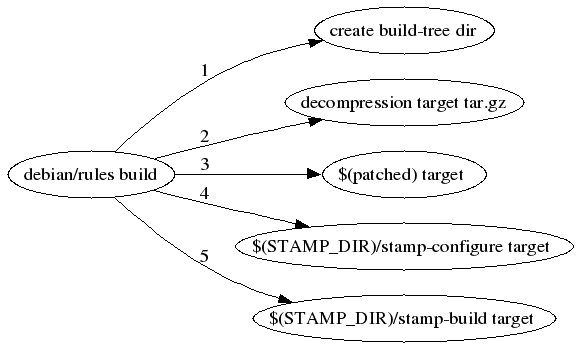
\includegraphics{image200702/dbs00.png}

\begin{enumerate}
\item create build-tree ディレクトリ \\
	\$BUILD\_TREE で指定されたディレクトリを作成します。
	デフォルトでは {\bf build-tree} になっています。

\item decompression tar.gz \\
	ソースコードが圧縮されている tar.gz を build-tree ディレクトリに解凍します。

\item \$(patched) target  \\
	debian/patches ディレクトリにあるパッチを適用します。

\item \$(STAMP\_DIR)\/stamp-configure target \\
	stamp-configure ターゲットを実行します。
	hello-dbs では \$BUILD\_TREE ディレクトリに移動し、configure を実行します。

\item \$(STAMP\_DIR)/stamp-build target \\
	stamp-build ターゲットを実行します。
	hello-dbs では \$BUILD\_TREE ディレクトリに移動し、make を実行します。 
\end{enumerate}

build 時の dpatch との違いは、

\begin{itemize}
\item パッチを当てるためのターゲット名が異なる

	dpatch は patch-stampになりますが、dbs は \$(patched)です。\\
	\$(patched) は {\bf /usr/share/dbs/dbs-build.mk}内で \$(STAMP\_DIR)/patchapply と宣言されています。

\item マーク用のファイル名が異なる

	stamp-configure や stamp-build というマーク用のファイル名が逆だったりします。
	( dpatch は configure-stamp / build-stamp )
\end{itemize}


\subsubsection{パッケージのclean}
dbs の ソースのcleanターゲットはいたってシンプルです。
dpatch は 既に展開されているソースにパッチを適用するため、cleanターゲット時には適用されたパッチを外す処理が必
要になりますが、dbs では、build 時に生成されたマークファイル用ディレクトリやソース格納先ディレクトリ
(\$BUILD\_TREE)をばっさり削除します。これには、適用されたパッチの管理等を行わずに済むというメリットがあります。

しかし、dbs は パッケージビルド毎に 
\begin{enumerate}
	\item ディレクトリを削除
	\item tar.gz を解凍
	\item パッチ適用
\end{enumerate}
とするので、サイズの大きい tar.gz をパッケージ化するときは時間がかかるというデメリットもあります。

\subsection{パッチの変更}
dbs でパッチの変更を行うために以下のコマンドが提供されています。
\subsubsection{dbs-edit-patch}
	このコマンドは現在のソースからパッチを作成する環境を構築してくれます。
	hello-dbs で新しいパッチを作りたいという状況になったとします。
	以下のコマンドを実行します。

\begin{commandline}
% dbs-edit-patch  01mogeri_patch
\end{commandline}

	実行すると /tmp ディレクトリに 01mogeri\_patch というディレクトリが作成されます。
	ディレクトリの中は以下のようになっています。

\begin{commandline}
% ls -l /tmp/01mogeri_patch/
-rwxr-xr-x 1 iwamatsu iwamatsu  546 2007-02-15 06:00 dbs-update-patch
drwxr-xr-x 2 iwamatsu iwamatsu 1024 1996-08-04 23:48 hello-1.3.orig
drwxr-xr-x 2 iwamatsu iwamatsu 1024 1996-08-04 23:48 hello-1.3.orig-old
\end{commandline}

	hello-1.3.orig は修正対象のディレクトリで、hello-1.3.orig-old は修正前のディレクトリです。
	hello-1.3.orig を修正した内容と hello-1.3.orig-old で差分を取り、
	パッチを生成し、パッチをコピーしてくれるスクリプトが dbs-update-patch になっています。
	
\begin{commandline}
#!/bin/sh -e
cd "/tmp/01mogeri_patch"
HOOK_DIR=/home/iwamatsu/dev/debian/dbs/hello-dbs-1.3/debian/dbs-hooks
test -d "$HOOK_DIR" && run-parts "$HOOK_DIR" --arg update-patch-prediff
find -name "*.bak" -print0 | xargs -0 --no-run-if-empty rm
find -name "*~" -print0 | xargs -0 --no-run-if-empty rm
: > new_patch
diff -ruN  hello-1.3.orig-old hello-1.3.orig >> new_patch || test $? -eq 1
mv new_patch "/home/iwamatsu/dev/debian/dbs/hello-dbs-1.3/debian/patches/01mogeri_patch"
test -d "$HOOK_DIR" && run-parts "$HOOK_DIR" --arg update-patch-postdiff
\end{commandline}
	
	例えば、

\begin{commandline}
cat  /tmp/01mogeri_patch/hello-1.3.orig/MOGERI
mogemogeri
\end{commandline}

	という修正を行い、{\bf /tmp/dbs-update-patch} を実行した場合、

\begin{commandline}
% /tmp/01mogeri_patch/dbs-update-patch
% ls -l debian/patches/01mogeri_patch
-rw-r--r-- 1 iwamatsu iwamatsu 212 2007-02-15 06:08 debian/patches/01mogeri_patch
% cat debian/patches/01mogeri_patch
diff -ruN hello-1.3.orig-old/MOGERI hello-1.3.orig/MOGERI
--- hello-1.3.orig-old/MOGERI   1970-01-01 09:00:00.000000000 +0900
+++ hello-1.3.orig/MOGERI       2007-02-15 06:06:54.000000000 +0900
@@ -0,0 +1 @@
+mogemogeri
\end{commandline}

	となります。

\subsection{まとめ}
今回、dbs を触ってみたのですが、
\begin{itemize}
	\item ソースが見えない

		ソースが tar.gz で固まっているため、見ることができない。
		見るには コマンドを使って解凍する必要がある。

	\item dpatch と比べてソースの編集がしずらい

		コマンドは用意されているんだけど、一回 /tmp 等に持っていって修正して.... という
		作業が発生するので、めんどうくさいところがある。

\end{itemize}
	という感想です。また、dbs を使っていたパッケージも だんだん dpatch に移行しつつあるので
	もう役目は追えたのではないかという気もします。

\dancersection{darcs 使いかた}{David Smith}
\label{sec:darcs}

darcsはソースコード管理ツールの一つです。Haskellで開発されている注目プロ
ジェクトとしてEmacs、Common Lisp、そしてHaskellのコミュニティでは大好評で
す。\footnote{大好評は多分言い過ぎです。せいぜい部分的に気に入られていま
す。}

git、Mercurial、monotone、他の数多くの分散ソース管理ツールの仲間であ
ります。しかし、gitなどの分散ソース管理ツールと違い、バージョンは管理しな
く、パッチを管理します。その二つの理念の違い、つまりバージョン管理対パッ
チ管理、についてdarcsを活用しながら説明します。

\subsection{基本なdarcs}

\subsubsection{とりあえず使ってみよう}

先ず、新規リポジトリを作ってみます。

\begin{commandline}
exponent,1102:~/workspace> mkdir myproject
exponent,1103:~/workspace> cd myproject
exponent,1104:~/workspace/myproject> darcs ini
exponent,1105:~/workspace/myproject> ls
_darcs
exponent,1106:~/workspace/myproject> echo 'Hello Darcs!' > README
exponent,1107:~/workspace/myproject> darcs whatsnew
No changes!
exponent,1108:~/workspace/myproject> darcs add README
exponent,1109:~/workspace/myproject> darcs whatsnew
\{
addfile ./README
hunk ./README 1
+Hello Darcs!
\}
exponent,1110:~/workspace/myproject> darcs record
Darcs needs to know what name (conventionally an email address) to use as the
patch author, e.g. 'Fred Bloggs <fred@bloggs.invalid>'.  If you provide one
now it will be stored in the file '_darcs/prefs/author' and used as a default
in the future.  To change your preferred author address, simply delete or edit
this file.\footnote{残念ながら、国際化はまだまだ出来ていません。}

What is your email address? David Smith <davidsmith@acm.org>
addfile ./README
Shall I record this change? (1/?)  [ynWsfqadjkc], or ? for help: y

hunk ./README 1
+Hello Darcs!
Shall I record this change? (2/?)  [ynWsfqadjkc], or ? for help: y

What is the patch name? Say hello to darcs
Do you want to add a long comment? [yn]n

Finished recording patch 'Say hello to darcs'
exponent,1111:~/workspace/myproject> darcs changes
Fri Apr 20 15:43:45 JST 2007  David Smith <davidsmith@acm.org>
  * Say hello to darcs
\end{commandline}

darcsではリポジトリの状態はパッチ集合だけで成り立ちます。パッチ
を作るのはファイルをdarcsに登録し、内容を記録し、最後に名前付けで完成し
ます。ちなみにパッチは名前だけで識別され、バージョン番号は一切ありません。
\footnote{自分の名前とメール先を\$HOME/.darcs/authorに書いたら聞かれませ
ん。}

\begin{tabular}{|l|l|p{15em}|l|}
\hline
\hline
コマンド名 & 例 & 意味\\
\hline
init & darcs init & 
 リポジトリを初期化する\\
\hline
whatsnew & darcs whatsnew -v &
 現在のリポジトリと記録済みの情報との差分を明示する\\
\hline
record & darcs record -m 'バグ\#103を修正' &
 パッチをリポジトリに記録する\\
\hline
changes & darcs changes --summary &
 パッチによるチェンジログを生成する\\
\hline
add & darcs add realcsh.c &
 新しいファイルをdarcsに教える\\
mv & darcs mv realcsh.c dangershell.c &
 ファイル名前変更\\
\hline
\hline
\end{tabular}

\subsubsection{他のリポジトリとの同期}

darcsはリポジトリ内のブランチをサポートしていません。複数リポジトリに同じパッ
チを一個も共有すれば、ブランチと呼んでもいいとのことです。つまり、リポジ
トリのコピーしかブランチが作れません。darcs getで既に存在するロカールリポ
ジトリ又はネットワークを通して取得出来るリポジトリでコピーできます。
\footnote{現在、HTTP及びSSHのみの通信になっています。}もちろん、ローカル
の場合にgetを使わずcpでも大丈夫です。

\begin{commandline}
exponent,1049:~/workspace> darcs get myproject myproject2
Copying patch 1 of 1... done!
Finished getting.
exponent,1050:~/workspace> cd myproject2
exponent,1051:~/workspace/myproject2> echo 'Darcs rules!' >> README
exponent,1052:~/workspace/myproject2> darcs record -m 'Add more darcs love'
hunk ./README 2
+Darcs rules!
Shall I record this change? (1/?)  [ynWsfqadjkc], or ? for help: y

Finished recording patch 'Add more darcs love'
exponent,1054:~/workspace/myproject2> darcs push ../myproject

Fri Apr 20 18:04:37 JST 2007  David Smith <davidsmith@acm.org>
  * Add more darcs love
Shall I push this patch? (1/1)  [ynWvpxqadjk], or ? for help: y

Finished applying...

exponent,1055:~/workspace/myproject2>
\end{commandline}

この時、先方のリポジトリに書き込み権利がありましたが、公開されている一般
的なプロジェクトでは開発者以外はコミット出来ないでしょう。そのため、
push/pullの代わりにsend/applyを使います。sendは指定するパッチをメールで送
り、applyはファイルにあるdarcs形式パッチをリポジトリに記録します。

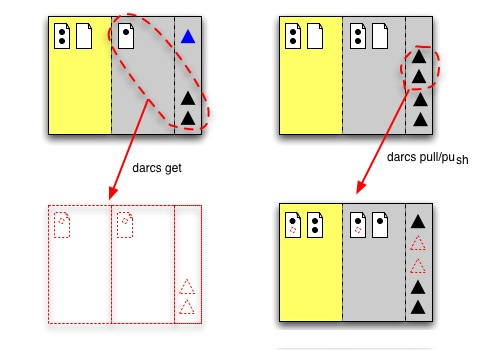
\includegraphics{image200704/darcs/pushpull.jpg}

ここまでdarcsの機能がほとんど普通だと言えるでしょう。しかしながら
パッチとパッチの依存関係を計算するための「パッチ代数」により
Cherry Picking(桜取り)というワークフローが他より余程手軽に
できます。残念ですが、例を造るのにdarcsが無限ループに落ちているばかり
のようなので、とにかく素晴らしいと信用してください。

\subsubsection{darcs-buildpackage}

Debianパッケージ支持とHaskellを習うためにJohn Goerzenさんが
darcs-buildpackageを開発しました。現在、ほとんどソース管理ツールでは
Debianパッケージ作業のための'-buildpackage'パッケージはあるよう、
その中でdarcs-buildpackageの使い方も同様ですので共通できます。

残念ながら、darcsは実際にリポジトリサイズに対して動作がとても
遅くなることがあったり、小さいリポジトリでもパッチ代数問題の解決
のため、ものすごく負荷かかりることもあります。
darcsの上流開発はgitとMercurialと比べると活発とは言えませんが、
理論的にリポジトリの内容に一切障害を与えなく最適化が
着々と行われています。私としては機能が改善するはずだと思いますが
Mercurialに大抵負けています。\footnote{John Goerzenさんも既にdarcsよりhg
に変更しました}

\dancersection{git-buildpackage の使いかた}{上川 純一}
\label{sec:git}

git はソースコードを管理するためのツールです。ソースコード管理のツール、
もしくはバージョン管理ツールと呼ばれ、VCSやSCMなどと略称されるツールのひ
とつです。また、旧来のCVS、SVNなどの集中モデルのSCM と違い分散モデルを採
用しているため、分散SCM(DSCM)と呼ばれます。 そのgitを利用してDebianのパッ
ケージを管理するための仕組が git-buildpackage です。

git-buildpackage 利用の詳細に入る前に、基本的な git の利用方
法を紹介します。

\subsection{git超入門}

\subsubsection{git でのデータの流れ}

まず最初に git で管理している場合のデータの流れをみてみましょう。各利用者が
直接編集しているデータが git-commit や git-push / git-pull コマンドでや
りとりされます。\footnote{本当はローカルレポジトリとリモートレポジトリの
区別はないため、技術的には直接ユーザ間でのgit-pull/git-push が可能です。}

\includegraphics[width=0.8\hsize]{image200704/git-repos.eps}

\subsubsection{git 関連用語}

ここで、この文書で利用する関連用語を整理しておきます。

\begin{tabular}{|l|p{30em}|}
\hline
\hline
用語 & 定義 \\
\hline
 ワーキングツリー & SCMで管理されている作業用のディレクトリで、ユーザが
 直接作業できるようにファイルがある場所\\
\hline
 ローカルレポジトリ & SCMで管理されているデータ
 ワーキングツリーと同じ場所の
 .git ディレクトリに実体がある。直接ファイルを編集することはできない\\
\hline
 リモートレポジトリ & SCM管理されているデータで、
 ネットワーク上のどこかに存在し
 ているもの。しばしば他人と共有している。直接ファイルを編集することはで
 きない
 \footnote{技術的、データ構造的にはローカルレポジトリとリモートレポジト
 リに大きな違いはないが説明する便宜上分類する。}\\
\hline
 コミット & ワーキングツリーからローカルレポジトリに情報を反映すること\\
\hline
 プッシュ & ローカルレポジトリからリモートレポジトリに情報を反映するこ
 と\\
\hline
 プル & リモートレポジトリからローカルレポジトリとワーキングツリーに情報を反映するこ
 と\\
\hline
\hline
\end{tabular}
\subsubsection{git でよく使うコマンド}

git\footnote{Debian では {\tt apt-get install git-core} でインストールで
きる} の基本的な操作はコマンドラインプログラムで実行できるようになってい
ます。gitパッケージは多数のコマンドラインのプログラムで構成されています。
多数のコマンドはありますが、実は毎日のオペレーションに必要なもの、特に既
存の別の SCM から移行してきた場合にいままで行ってきたことと同じことをす
るために必要なものというのはそれほど多くありません。git でよく使うコマン
ドを解説します。

\begin{tabular}{|l|l|p{15em}|l|}
\hline
\hline
コマンド名 &例 &意味 & cvs 相当\\
\hline
git-clone & git-clone {\it git://XXX/YYY} & 
 リモートレポジトリをローカルにクローンし、ワーキングツリーをチェックアウトする & cvs login, cvs co \\
\hline
git-init-db & git-init-db &
 ローカルレポジトリ(.gitディレクトリ)を作成する & cvs init\\
\hline
git-pull & git-pull {\it git://XXX/YYY} &
 リモートレポジトリの変更をローカルにマージし、ワーキングツリーを
 アップデートする & cvs up \\
\hline
git-commit & git-commit -a -m 'xxx' & 
 ローカルレポジトリに変更をコミットする & cvs ci の前半\\
\hline
git-push & git-push {\it git://XXX/YYY} & 
 ローカルレポジトリをリモートレポジトリに送信する & cvs ci の後半\\ 
\hline
git-add & git-add {\it filename}&
 ファイルを次回コミットの際にローカルレポジトリに追加されるように登録す
 る & cvs add \\
\hline
git-rm & git-rm {\it filename} & 
 ファイルを次回コミットの際にローカルレポジトリから削除されるように登録す
 る & cvs remove \\
\hline
git-status & git-status & 
 ローカルレポジトリに対してワーキングツリーの状況を確認する &
 cvs status\\
\hline
git-diff & git-diff & ローカルレポジトリとワーキングツリーの差分を
 表示する & cvs diff\\
\hline
\hline
\end{tabular}

\subsubsection{よくある作業の流れ}

\begin{minipage}{0.5\hsize}
よくある作業の例を紹介します。

まず、新しくローカルレポジトリをつくるのであれば、git-init-db でローカルレポジトリを作成
し、ファイルをgit-add, git-commit で追加します。そうでなければ、既存のリ
モートレポジトリを git-clone で複製します。これで、作業可能なワー
キングツリーができ、 .git ディレクトリにはローカルレポジトリが作
成されました。

ワーキングツリーでファイルを編集して、git-commit でローカルレポジトリに反
映します。削除・追加がある場合には、git-add/git-rmコマンドを利用します。
通常は、何がコミットされるのか、を git-status コマンドで確認し、ファイル
を指定してコミットすることになるでしょう。git-diff コマンドでこれからコ
ミットする予定の差分を確認することもできます。

リモートレポジトリと同期するため、まず git-pull で最新の情
報を取得します。ここでコンフリクトがあればワーキングツリーを修正し、git-commit します。
問題ないようであれば、git-push でリモートレポジトリに送信します。
\end{minipage}
\begin{minipage}{0.5\hsize}
\includegraphics[width=1\hsize]{image200704/git-work.eps}
\end{minipage}

\subsubsection{GUIツール}

\begin{minipage}[b]{0.5\hsize}
git の履歴情報などを見るのには、視覚的にわかりやすい Qt の GUI である 
 qgit\footnote{apt-get install qgit でインストール可能} を利用すると履歴
 や差分が見れて便利です。GUIが利用できない環境では、git-whatchanged コマ
 ンドなどを利用すればよいでしょう。他のGUIとして git-gui \footnote{旧
 gitkがgit-gui にリネームされた, apt-get install git-gui でインストール
 可能}や、gitweb \footnote{ウェブフロントエンドapt-get install gitwebで
 インストール。}があります。

コミットに特化したツールとして、gct\footnote{apt-get install gct} なども
 あります。

\end{minipage}
\begin{minipage}[c]{0.5\hsize}
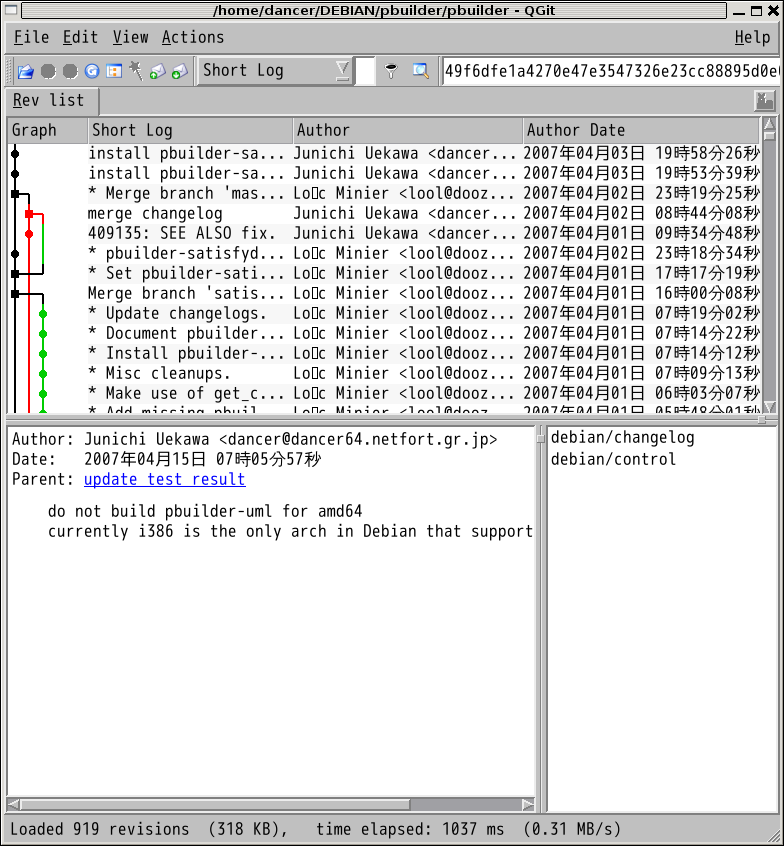
\includegraphics[width=0.8\hsize]{image200704/qgit.png}
\end{minipage}

\subsection{git-buildpackage の流れ}

git-buildpackage\footnote{apt-get install git-buildpackage でインストー
ル可能} を利用した場合のパッケージングの流れを紹介します。前提として、 
upstream では謎の利用不可能なSCMを利用して開発をすすめており、Debian
Developerはリリース毎に出てくる tar-ball しか利用できないものとします。

\includegraphics[width=1\hsize]{image200704/git-buildpackage.eps}

\subsubsection{git-import-dsc}

まず、Debian Developerはアップストリームの tarball を展開し、
そこで dh\_{}makeを実行し、一連のパッケージング作業を行います。

\begin{commandline}
[14:10:52]dancer64:work> cp ../upstream/vvv-0.1.tar.gz .
[14:10:57]dancer64:work> 
[14:11:03]dancer64:work> tar xfz vvv-0.1.tar.gz 
[14:11:08]dancer64:work> cd vvv-0.1
[14:11:12]dancer64:vvv-0.1> dh_make -f ../vvv-0.1.tar.gz 

Type of package: single binary, multiple binary, library, kernel module or cdbs?
 [s/m/l/k/b] s

Maintainer name : Junichi Uekawa
Email-Address   : dancer@debian.org 
Date            : Sat, 14 Apr 2007 14:11:28 +0900
Package Name    : vvv
Version         : 0.1
License         : blank
Type of Package : Single
Hit <enter> to confirm: 
Done. Please edit the files in the debian/ subdirectory now. You should also
check that the vvv Makefiles install into $DESTDIR and not in / .
[14:14:44]dancer64:vvv-0.1> debuild -us -uc 
 fakeroot debian/rules clean
dh_testdir
dpkg-buildpackage (debuild emulation): full upload (original source is included)
Now running lintian...
W: vvv: binary-without-manpage usr/bin/hello-world.sh
W: vvv: script-with-language-extension usr/bin/hello-world.sh
E: vvv: helper-templates-in-copyright
E: vvv: description-is-dh_make-template
W: vvv: wrong-bug-number-in-closes l3:#nnnn
E: vvv: section-is-dh_make-template
Finished running lintian.
[14:16:51]dancer64:vvv-0.1> cd ..

[14:17:42]dancer64:work> ls
vvv-0.1		vvv_0.1-1.diff.gz  vvv_0.1-1_amd64.build    vvv_0.1-1_amd64.deb
vvv-0.1.tar.gz	vvv_0.1-1.dsc	   vvv_0.1-1_amd64.changes  vvv_0.1.orig.tar.gz
\end{commandline}

すると、Debianのソースパッケージファイルなどができます。

git-import-dsc は dsc ファイルをオプションにとると、[パッケージ名]ディレ
クトリを作成し、その中に git のローカルレポジトリを作成し、upstream と master ブラ
ンチ(通常利用するブランチ)を作成し、upstreamにアップストリームのツリーを
入れ、master に debian への改変を加えた後のツリーを入れます。この状態で、
git-buildpackage などでパッケージがビルドできる状態になっています。

\begin{commandline}
[14:17:42]dancer64:work> git-import-dsc vvv_0.1-1.dsc 
Upstream version: 0.1
Debian version: 1
Initialized empty Git repository in .git/
Created initial commit b7e3ddd5bb1033c2cd9ae90d86ea8b6f55fb34be
 3 files changed, 16 insertions(+), 0 deletions(-)
 create mode 100644 Makefile
 create mode 100644 hello-world.sh
 create mode 100755 orig.sh
dpkg-source: warning: extracting unsigned source package (/home/dancer/tmp/git-test/work/vvv_0.1-1.dsc)
dpkg-source: extracting vvv in /home/dancer/tmp/git-test/work/tmpwJLVOR/unpack/vvv-0.1-1
dpkg-source: unpacking vvv_0.1.orig.tar.gz
dpkg-source: applying /home/dancer/tmp/git-test/work/vvv_0.1-1.diff.gz
 VCSCMD:  git
LOGTEXT Imported vvv-0.1-1
into Git repository

Created commit 041935d50363f69bcb7ff1b5e0df43b79784b6b1
 9 files changed, 149 insertions(+), 2 deletions(-)
 create mode 100644 debian/README.Debian
[中略]
 create mode 100755 debian/rules
[14:17:58]dancer64:work> cd vvv
[14:18:09]dancer64:vvv> git-status
# On branch master
nothing to commit (working directory clean)
[14:18:12]dancer64:vvv> git-branch
* master
  upstream
\end{commandline}

\subsubsection{git-import-orig}

新しいアップストリームのバージョンがリリースされた場合には、
git-import-dsc で作成されたディレクトリの中で git-import-orig コマンドを
実行して、ローカルレポジトリにインポートします。

\begin{commandline}
[14:18:50]dancer64:vvv> git-import-orig ../../upstream/vvv-0.2.tar.gz -u 0.2 
Upstream version is 0.2
Repository has uncommitted changes, commit them first: 
# On branch master
# Untracked files:
#   (use "git add <file>..." to include in what will be committed)
#
#	build-stamp
#	configure-stamp
#	debian/files
#	debian/vvv/
nothing added to commit but untracked files present (use "git add" to track)

[14:19:04]dancer64:vvv> debclean 
Cleaning in directory ./.git/refs/tags
Directory ./.git/refs/tags: contains no debian/changelog, skipping
Cleaning in directory .
dh_testdir
dh_testroot
rm -f build-stamp configure-stamp
# Add here commands to clean up after the build process.
/usr/bin/make clean
make[1]: ディレクトリ `/home/dancer/tmp/git-test/work/vvv' に入ります
make[1]: `clean' に対して行うべき事はありません.
make[1]: ディレクトリ `/home/dancer/tmp/git-test/work/vvv' から出ます
dh_clean 
[14:19:28]dancer64:vvv> git-import-orig ../../upstream/vvv-0.2.tar.gz -u 0.2 
Upstream version is 0.2
Importing ../../upstream/vvv-0.2.tar.gz to upstream branch...
Switched to branch "upstream"
  master
* upstream
 VCSCMD:  git
LOGTEXT Imported vvv-0.2
into Git repository



Created commit 8e61554f99a28de9b10c23ae0319b8cc4aa07b40
 2 files changed, 4 insertions(+), 1 deletions(-)
 create mode 100644 NEWS
Merging to master
Switched to branch "master"
* master
  upstream
 100% (14/14) done
Auto-merged Makefile
CONFLICT (content): Merge conflict in Makefile
Automatic merge failed; fix conflicts and then commit the result.
git-pull returned 1
Couldn't pull upstream to .
Import of ../../upstream/vvv-0.2.tar.gz failed
[14:19:50]dancer64:vvv> cat Makefile 
all:

install:
<<<<<<< HEAD:Makefile
	install -o root -g root -m 755 hello-world.sh $(DESTDIR)/usr/bin/hello-world.sh
=======
	install -o root -g root -m 755 hello-world.sh /usr/local/bin/hello-world.sh
>>>>>>> 8e61554f99a28de9b10c23ae0319b8cc4aa07b40:Makefile

clean:

.PHONY: all install clean

[14:19:58]dancer64:vvv> vi Makefile
[14:20:15]dancer64:vvv> git-commit -a -m '0.2 debian changes'
Created commit cffcdabb818fdacc38f1a21bab744c56480d1a44
\end{commandline}

この操作により、upstream ブランチに新しいバージョンがインポートされ、
master ブランチに変更がマージされ、適切なタグが作成されます。

\subsubsection{git-buildpackage}

各種編集を行い、コミットを完了したら、git-buildpackage を実行し、レポジ
トリの内容から Debian パッケージを作成します。--git-tag オプションを付け
ておくとビルドしなおしたら適切なタグを自動でつけてくれるので便利です。
また、コミットしわすれていると警告を出してくれるのもよいです。

\begin{commandline}
[14:21:26]dancer64:vvv> git-buildpackage 
[中略]
You have uncommitted changes in your source tree:
# On branch master
# Changed but not updated:
#   (use "git add <file>..." to update what will be committed)
#
#	modified:   debian/changelog
#
no changes added to commit (use "git add" and/or "git commit -a")

Use --git-ignore-new to ignore.
[14:21:34]dancer64:vvv> git-commit -a -m 'update changelog'
Created commit 98ae75017264f86192d30b894191d862b98821f5
 1 files changed, 6 insertions(+), 0 deletions(-)
[14:21:43]dancer64:vvv> git-buildpackage 
dh_testdir
dh_testroot
rm -f build-stamp configure-stamp
[中略]
$ git-buildpackage -us -uc --git-tag
\end{commandline}
%$

\subsection{アップストリームが git で管理している場合}

別のシナリオを考えてみます。アップストリームが git で管理している場合に
直接 git を利用したワークフローは幾分か簡単にできます。
どちらがよいかはわかりませんが、参考までに掲載します。

git-clone したらローカルレポジトリはリモートレポジトリから見たらただのブランチ
のため、ローカルレポジトリで変更を加えていれば、
git-pull するたびにアップストリームの変更をマージすることになります。
ビルドする際には、debuild などを直接使えばよいでしょう。ただ、
この場合は自動でタグをつけたりはしてくれません。

\begin{commandline}
$ debuild -us -uc -i -I 
\end{commandline}
%$

そのため、git-import-dsc, git-import-orig を使わない場合においても
git-buildpackage を利用するのがよいでしょう。upstream ブランチが必要にな
るのは git-import-orig をする際だけなので、master ブランチのみしかなく
ても動きます。

\begin{commandline}
$ git-buildpackage -us -uc -i -I 
\end{commandline}

\includegraphics[width=1\hsize]{image200704/git-clone.eps}

\dancersection{git の実装技術的解説}{上川 純一}

簡単にgit のレポジトリ\footnote{ローカルレポジトリもリモートレポジトリも
基本的には同じファイル構成です。}のファイル構成のコンセプトを紹介します。
レポジトリのファイルは .git ディレクトリ以下\footnote{もしくは環境変数 
GIT\_{}DIR で指定された場所}にあります。基本的なオブジェクトは commit,
tree, blob の三種類があります。.  git/objects/ 以下にファイルはgzip 圧縮
された状態で保存されています。.  git/HEAD (最近は 
.git/refs/heads/master) に最新の commit のハッシュ(ハッシュはデータの
sha1sumをとることで取得している)が記録されています。commit の中身を見る
と、tree のハッシュと 親 commit とコミットメッセージ情報が含まれています。
treeを見ると、そのコミットのときのディレクトリ情報が含まれており、それぞ
れのファイル実体(blob)の hash 値が含まれています。

なお、objects はばらばらで管理されるとディスクの利用効率が悪いので
git-repack コマンドを利用して pack 形式で保存されることが多いです。そう
なると、.git/objects/pack に保存されます。

\includegraphics[width=0.38\hsize]{image200704/git-filesystem-concept.eps}
\includegraphics[width=0.5\hsize]{image200704/git-filesystem-concept2.eps}

この情報を具体的にコマンドラインで確認してみた例を例示します。特に重要な
点は、'head'ファイルへの書き込みというOS観点ではアトミックに実装できるオ
ペレーションでコミットが実現されているということでしょう。\footnote{ファ
イルの SHA-1 ハッシュ値の衝突が発生しないということが前提です。ただ、現
実的に問題になることは無いでしょう。}

\begin{commandline}
[11:39:25]dancer64:pbuilder> cat .git/refs/heads/master
49f6dfe1a4270e47e3547326e23cc88895d0e05d
[11:39:38]dancer64:pbuilder> git-cat-file -t 49f6dfe1a4270e47e3547326e23cc88895d0e05d
commit
[11:39:44]dancer64:pbuilder> git-cat-file commit 49f6dfe1a4270e47e3547326e23cc88895d0e05d
tree 98dc4f51c0ae895607db43f8b617a7cacfbdc34b
parent e40c851b3017b09a609e2e36af6ae8a20b8ffff3
author Junichi Uekawa <dancer@dancer64.netfort.gr.jp> 1176588357 +0900
committer Junichi Uekawa <dancer@dancer64.netfort.gr.jp> 1176588357 +0900

do not build pbuilder-uml for amd64
currently i386 is the only arch in Debian that supports user-mode-linux
[11:39:47]dancer64:pbuilder> git-cat-file -t 98dc4f51c0ae895607db43f8b617a7cacfbdc34b
tree
[11:39:52]dancer64:pbuilder> git-cat-file tree 98dc4f51c0ae895607db43f8b617a7cacfbdc34b|strings|head -5
100644 .cvsignore
100644 .gitignore
100644 AUTHORS
o[v'a
R100644 COPYING
[11:40:13]dancer64:pbuilder> git-ls-tree 98dc4f51c0ae895607db43f8b617a7cacfbdc34b|head -5
100644 blob 99ee691a57a1d79999965e8f9362da79d18e8ce4    .cvsignore
100644 blob e4e5f6c8b2deb54bf38312dd9e2f53489b60d6a6    .gitignore
100644 blob 30ded29ac4176f5b7627618b27a8cb15c7ea0a52    AUTHORS
100644 blob b7b5f53df1412df1e117607f18385b39004cdaa2    COPYING
100644 blob 97cae37dd0355d4f29837bc02bbad4bcdba98914    ChangeLog
[11:40:18]dancer64:pbuilder> git-cat-file -t 97cae37dd0355d4f29837bc02bbad4bcdba98914
blob
[11:40:36]dancer64:pbuilder> git-cat-file blob 97cae37dd0355d4f29837bc02bbad4bcdba98914|head
2007-04-11  Junichi Uekawa  <dancer@debian.org>

        * AUTHORS, etc: remove $Id$, which is CVS specific

2007-04-10  Junichi Uekawa  <dancer@debian.org>

        * Documentation/pbuilder-doc.xml: update documentation

        * pbuilder-modules: say lenny instead of sarge

[11:40:43]dancer64:pbuilder> ls .git/objects/97/cae37dd0355d4f29837bc02bbad4bcdba98914
.git/objects/97/cae37dd0355d4f29837bc02bbad4bcdba98914
[11:40:58]dancer64:pbuilder> ls -l .git/objects/97/cae37dd0355d4f29837bc02bbad4bcdba98914
-r--r--r-- 1 dancer dancer 27255 2007-04-11 09:01 .git/objects/97/cae37dd0355d4f29837bc02bbad4bcdba98914
\end{commandline}


\dancersection{仮想マシンモニタKVM}{上川 純一}
\label{sec:kvm}

KVM という仮想マシンモニタがあります。これは、 Intel VT, もしくは、AMD-V 
対応のプロセッサ\footnote{Intel Core Duoや、Opteron Rev. Fなど} の仮想化
対応機能を活用するための仕組です。2006年末の時点では、kvmはデバイスドラ
イバとして実装されており、 \texttt{/dev/kvm}として実装されています。


\subsection{使いかた}

\begin{wrapfigure}{r}{5cm}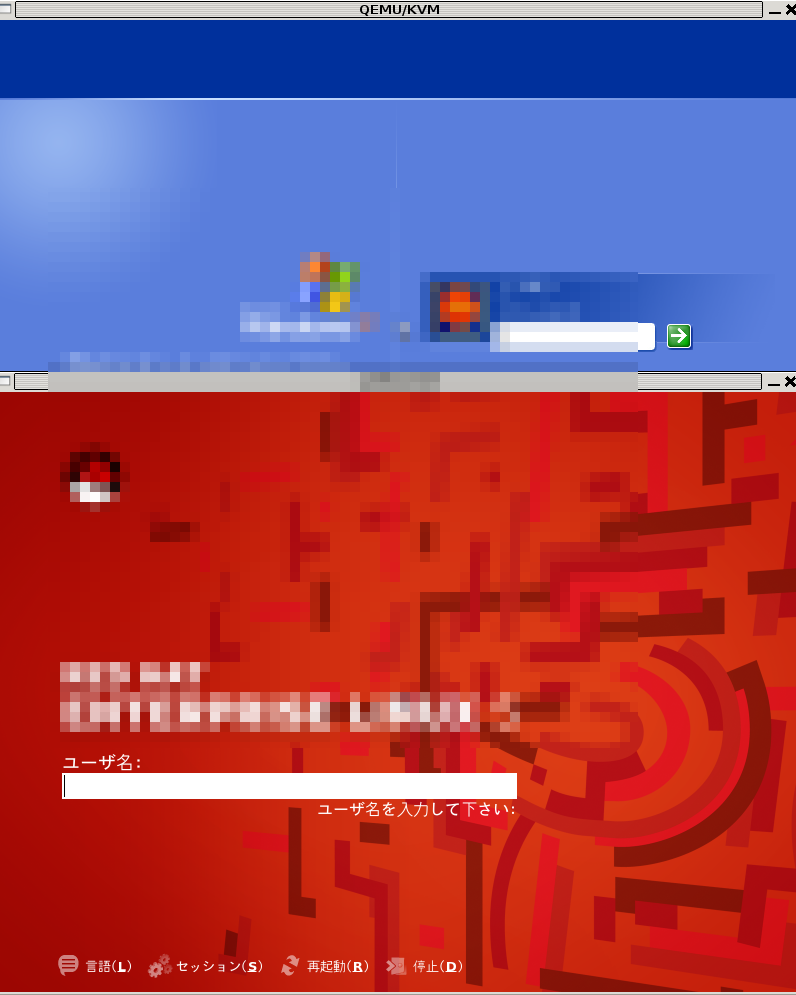
\includegraphics[width=5cm]{image200701/kvm.png}\end{wrapfigure}

Linus Kernel 2.6.20 以降ではカーネル側の機構は標準で入っているようです。
\footnote{2.6.20-rc1 で導入され、まだ 2.6.20 はリリースされていないため
この記事の内容は1月19日時点での予測です} Debian で KVM を利用する際の手
順を説明します。

\texttt{apt-get install kvm} でパッケージをインストールします。kvm コマ
ンドがインストールされます。これが kvm 向けに変更された qemu です。

udev が作成してくれる \texttt{/dev/kvm} にアクセスできるようにします。 
デフォルトは\texttt{ root:kvm 660}\footnote{バージョン11-1以降の場合} で、rootのみがアクセスできる設定になっ
ています。ユーザを kvm グループに追加すればよいでしょう。

\begin{commandline}
# adduser dancer kvm
\end{commandline}

CPUのVT機能はデフォルトで on になっていない場合があるので、 on にします。
これはマシンによって違うようです。 通常 BIOS で設定します。 旧モデルの MacBook の場
合は EFI 上で必要なコマンドを発行することになります。
\footnote{\texttt{vmx-var-set.efi}という名前で流通しているようです。}

以上で、kvm コマンドを利用してVTの恩恵にあずかることができるようになりま
す。コマンドラインなどはqemu 互換、むしろ qemu そのものを利用しているの
で、qemu と同じように動かすことができます。


\subsection{実行例}


kvm を活用していろいろと試してみましょう。qemu 用のディスクイメージを作
成し、適当なディストリビューションのディスクイメージを利用して、インストー
ルします。おそらく、-monitorコマンドで stdio をモニタにするほうが便利で
しょう。

\begin{commandline}
$ qemu-img create -f qcow hda 10G
$ kvm -hda hda -cdrom /home/iso/RHEL4-U4-i386-AS-disc1.iso
   -boot d -m 512 -monitor stdio
(qemu) change cdrom /home/iso/RHEL4-U4-i386-AS-disc2.iso
(qemu) change cdrom /home/iso/RHEL4-U4-i386-AS-disc3.iso
(qemu) change cdrom /home/iso/RHEL4-U4-i386-AS-disc4.iso
(qemu) change cdrom /home/iso/RHEL4-U4-i386-AS-disc5.iso
(qemu) change cdrom /home/iso/RHEL4-U4-i386-AS-disc1.iso
(qemu) eject cdrom
\end{commandline}

ここでは某CDROMが5枚あるディストリビューションを例にとっていますが、
CDROMが5枚あっても、qemu モニターにてCDROMを入れ換えながらGUI操作を行う
ことで無事にインストール完了します。リブートするところでゲストOSがカーネ
ルパニックを起こしますが、そこは適当に kvm 自体を起動しなおせば問題あり
ません。

\begin{commandline}
$ kvm -hda hda  -boot c -m 512 -monitor stdio -localtime  \
 -redir tcp:2222::22
\end{commandline}


\subsection{ベンチマークしてみた}

qemu を使った場合と kvm を使った場合の速度比較をしてみました。まず、ユー
ザ空間で完結する例として単純に while でループを回すだけのプログラムです。
qemu の場合は 6s かかったものが、 kvm の場合は 0.6s で完了しました。

\subsection{パフォーマンスの見えかた}

kvm を実行しているホストOSからどのように見えるのか確認してみましょう。
kvm の仕組だと、システムコールを実行して処理を行うことになるのでしょう。

\texttt{mpstat -P ALL 1} の出力を一部みてみると、一つのCPUの システム時
間がとられているように見えます。

\begin{commandline}
00時28分51秒  CPU   %user   %nice    %sys %iowait    %irq   %soft  %steal   %idle    intr/s
00時28分52秒  all    0.00    0.00   50.00    0.50    0.00    0.50    0.00   49.00   1421.78
00時28分52秒    0    0.00    0.00   92.08    0.00    0.00    0.99    0.00    6.93    430.69
00時28分52秒    1    0.00    0.00    6.93    0.99    0.00    0.00    0.00   91.09    991.09
\end{commandline}

\texttt{top}コマンドで見た場合には、kvmは通常のプロセスと同様にCPU時間を
消費し、メモリを消費しているように見えます。

\begin{commandline}
  PID USER      PR  NI  VIRT  RES  SHR S %CPU %MEM    TIME+  COMMAND
 3746 dancer    25   0  308m 252m 246m R   82 25.7 100:36.60 kvm
 2512 root      10  -5     0    0    0 S    0  0.0   0:11.32 kjournald
 2806 root      15   0  2556  932  804 S    0  0.1   1:09.36 syslogd
\end{commandline}

\texttt{iostat 1 /dev/dm-1 }の出力を確認してみます。
ゲストOSのディスクIOによってホストOSのディスクIOが発生しているのが見れます。

\begin{commandline}
avg-cpu:  %user   %nice %system %iowait  %steal   %idle
           0.00    0.00   42.50   42.00    0.00   15.50

Device:            tps   Blk_read/s   Blk_wrtn/s   Blk_read   Blk_wrtn
dm-1            805.94       102.97      6400.00        104       6464
\end{commandline}

\subsection{他との比較}

Xen, qemu, qemu+kqemu, openvz, vserver, user-mode-linux などと機能を比較
してみましょう。と思ったらすでにやられていたので、このURLを参照してくだ
さい。\url{http://virt.kernelnewbies.org/TechComparison}


\dancersection{Bug Squashing Party}{岩松 信洋}
\subsection{はじめに}
今回 Debian JP Project で Bug Squashing Party を行いました。
その内容と報告をまとめました。
 
\subsection{Bug Squashing Party とは?}
Bug Squashing Party\footnote{http://wiki.debian.org/BSP} とはバグつぶし大会のことです。
Debian の場合だと、stable のリリース前や定期的に行われています。
目的としては Release Critical Bug を減らしたり問題のあるパッケージを集中的に直したりします。

\subsubsection{Bug Squashing Party の重要な点}

Bug Squashing Party は以下の点を決める事が重要です。
\begin{itemize}
	\item 日時

		Bug Squashing Party をやる日時と開催期間を決める必要があります。
	\item 場所

		Bug Squashing Party を行う場所を決める必要があります。
		IRC だけでなく、場所を借りて Face to Face で話合いながら
		行う必要もあるからです。 
	\item コーディネーターおよび指揮官
		
		Bug Squashing Party を円滑に進めるため、指揮官が必要です。
		バグの情報を把握し、参加者に指示を行います。
		Debian の場合だと、Debian Release Manager や Release チームと話を進める
		ことがあります。このような場合には Release チームに名前が知られている人に
		コーディネーターになってもらったほうが話が進めやすくなるかもしれません。
\end{itemize}

\subsubsection{コーディネイター、指揮官が行うこと}
コーディネイター、指揮官は、以下の事について知っている必要があります。
\begin{itemize}
	\item Bug Squashing Party の目的を把握する
		
		ただ単にバグを潰すだけではなく、今回はinput method に関してのバグを潰す、といった
		目的があると全体の流れをコントロールしやすいと思います。

	\item 他で行われている Bug Squashing Party の主催者やコーディネイターと話をする。

		他で Bug Squashing Party をやっている可能性があるので、話をして無駄な作業を減らすよう
		動く必要があります。

	\item バグ対策の指示

		参加者にバグの対策を指示します。
		
\end{itemize}

\subsubsection{参加者が事前に知っておくこと}

参加者はただ単にバグを潰すという作業をするだけではなく Bug Squashing Party はどのような
ものなのか理解しておく必要があります。

また、Debian の場合は NMU\footnote{Non Maintainer Upload} を行う可能性が高いので、NMU時の
パッケージバージョンの付け方やChangelog の書き方を知っておく必要があります。
もちろん Debian Policy なども事前に読んで勉強しておく必要があります。:-)


参加者の中で Debian Developer の方がおられる場合は、Debian Developer ではない人が修正した
パッケージのアップロードしたり、いろいろ助言等をしていただけると助かるかもしれません。

\subsection{今回行われた Bug Squashing Party }

\subsubsection{今回の Bug Squashing Party の目的}
今回の Bug Squashing Party の目的は以下のものがあります。

\begin{itemize}
	\item etch リリース前なので、RC バグを潰したい
	\item Bug Squashing Party ってどのようなものなのか、ためしにやってみる
	\item Debian JP Project はちゃんと活動しています、というアピール
\end{itemize}

\subsubsection{今回の Bug Squashing Party の流れ}

どのような流れ、内容でおこなったのか以下にまとめました。

\begin{enumerate}
\item 事の発端

 OSC 2006 の帰りにgotom さん、上川さん、えとーさん、小林さん、私でサイゼリアで食事していたところ、上川さんが
「Bug Squashing Party やりたいねぇ。」から始まったが、この時点でだれが話を進めることにするか決まらない。

\item Debian JP IRC ミーティングで議論

 Debian JP で行われたミーティングで、私が話を進めることになる。

\item debian-devel@debian.or.jp で提案

 Debian JP Project が提供している開発用メーリングリストで提案。\footnote{[debian-devel:16525] Bug Squashing Party について}
 この投稿によるスレッドで武藤さんから助言を頂く。

\item コーディネイターを決める

 Bug Squashing Party を進めるコーディネイターをして、gotomさんに依頼。
 快諾していだく。

\item 開催日時を決める
 
 ちょうど11/23 (木) が休みだったので、この日にする。朝弱い人のために10時から行うことにした。
 このあたりは IRC で決めた気がするが、ログがない。
 開催内容は以下のとおり。


\begin{commandline}

日時
        2006 年  11 月 23 日 (木) 10:00 - 15:00

会場
        IRC
	IRC サーバー	: osdn.debian.or.jp
	IRC チャンネル	: #debianjp-bsp
	漢字コード	: iso-2022-jp

コーディネイター
	後藤 正徳さん

\end{commandline}


\item 開催告知
 
 debian-users@debian.or.jp および debian-devel@debian.or.jp に開催告知を流した。
 しかし、反応なし。

\item 開催

 無事開催。しかし人の集まりが悪い。
 人が集まり始めると gotom さんがいろいろ指示をしてくれて、順調に Bug Squashing Party は進んだ。
 
 進めるにあたって、参考にしたサイトは以下のとおり。
 \begin{itemize}
  \item Debian RC バグ曲線 

	\url{http://bugs.debian.org/release-critical/}
  \item 現在の RC バグ情報 
	
	\url{http://bugs.debian.org/release-critical/debian/all.html}
  \item リリースチームが使っている RC バグ管理サイト 
	
\url{http://bts.turmzimmer.net/details.php}
 \end{itemize}
\item 終了

 15 時に終了。かなり不完全燃焼。
 NMU するまでが Bug Squashing Party です。

\end{enumerate}

\subsubsection{結果}
 今回行われた Bug Squashing Party の結果は以下の通りです。

\begin{itemize}
 \item 参加者\\
 gotom,
 iwamatsu,
 ay\_,
 Henrich,
 mino,
 dancerj,
 nori1,
 kmuto,
 omote\_bot,
 sato\_at\_deb-newb,
 tyuyu

 \item 活動内容
   \begin{itemize}
   \item xxdiff 修正 \debianbug{399764}
   \item qemu は問題なし \debianbug{399382}は close しても問題ない
   \item murasaki \debianbug{378318} hppa only
   \item libflash-mozplugin \debianbug{399508} arm/ia64 only
   \item rarpd \debianbug{395739}
   \item cowdancer \debianbug{384132}
   \item zoph \debianbug{398637}
   \item リリースノート追従
   \item po-debconf 更新
   \item rsjog
   \item bookview最新版ビルドしていま作業中、arm fix失敗
   \end{itemize}
\end{itemize}

\subsubsection{感想}

 Bug Squashing Party が終わったあと、IRC で意見交換を行いました。

\begin{itemize}

    \item 5時間は短い。重いバグが残っているので、簡単なバグフィックスではないので、終わらない。
    \item 普段手をかけていないアーキテクチャのマシンのアップデートだけで数時間かかる。 (普段から手をかけてメンテナンスしてあげましょう・・・)
    \item IRCですることに関しては問題ない。
    \item Bug Squashing Party とは、という説明がないので今後準備したいね。
    \item IRCなら参加していなくても、ちょくちょく様子がみられてうれしい。
    \item changelog に closed by Debian JP's BSP とか入れたほうがいいかも。

\end{itemize}

 これらの内容は\url{http://wiki.debian.org/BSP/DebianJP}としてまとめてあります。

\subsubsection{その他の Bug Squashing Party}
これは特に Debian だけの特別なイベント(行事?)ではなく、各ディストリビューションやプロジェクトで
行っています。
\begin{itemize}
	\item NetBSD
		
		The NetBSD Bugathon \url{http://www.netbsd.org/hackathon/} 
	\item OpenBSD

		hackathon \url{http://en.wikipedia.org/wiki/Hackathon}
	\item Gentoo

		Bug day \url{http://bugday.gentoo.org/} \\
		毎月第1土曜日は Bug day となっている。
	\item Gnome 

		Bug day \url{http://live.gnome.org/Bugsquad/BugDays}
\end{itemize}

俺一人 Bug Squashing Party を行ったりしている人もおられるようです。

\subsection{まとめ}
 今回、Bug Squashing Party 開催に関係したのですが、開催までは意外と簡単だったように思います。
 (協力者がたくさんおられたから、というのが一番大きいですが。)
 今回の開催時間は5時間と短かく、かなり中途半端でした。他の Bug Squashing Party では24時間とか
 平気でやっているようなので、今後は長い時間確保して行いたいと考えています。
 また、試験前の学生のようにならず、定期的に行っていけたらいいと考えています。


\dancersection{apt-torrent}{岩松 信洋}
\label{sec:apt-torrnet}

Debian パッケージのレポジトリを \texttt{bittorrent} ネットワーク上に置き、それを apt で取得するというものが \texttt{apt-torrent} です。

まだ Debian としては頒布されておらず、フランス人の方が一人でシコシコやっているようです。\url{http://sianka.free.fr/} で開発が行われています。

\subsection{bittorrent とは}
bittorrent とは、P2P を用いたファイル転送用プロトコルとその通信を行うソフトウェアの事を指します。
特徴としては、P2P でファイルの一部をお互いに送受信しあうというプロトコルになっているところです。

通常の P2P ソフトウェアではファイルを提供元に集まるようになっていますが、このプロトコルを使うこと
により、ネットワーク帯域のないピアもファイルの配布に協力できるようになっています。

このプロトコル上で Debian パッケージを頒布し、aptで取得するようにしたものが\texttt{apt-torrent}です。

\subsection{使い方}

\subsubsection{ダウンロード}
先にも書いたように Debian としては頒布されていません。
以下のサイトからダウンロードし、使用します。

\url{http://sianka.free.fr/download/apt-torrent_0.5.0-1_all.deb}

apt のソースとして利用できる apt-line も提供されており、以下の apt-line
を\texttt{/etc/apt/sources.list}に追記して使用可能です。
\begin{itemize}
	\item \url{deb http://sianka.free.fr/apt-torrent testing main}
	\item \url{deb-src http://sianka.free.fr/apt-torrent testing main}
	\item \url{deb http://sianka.free.fr/apt-torrent unstable main}
	\item \url{deb-src http://sianka.free.fr/apt-torrent unstable main}
\end{itemize}

\subsubsection{設定}
パッケージをインストールすると、自動的に \texttt{/etc/apt/sources.list} に追記されます。

以下が追加された \texttt{apt-torrent} 用の apt-line です。

\begin{commandline}
### BEGIN APT-TORRENT SOURCE LIST
# Do not edit or remove the markers, they are used by the apt-torrent package

# Uncomment one of the following:
# deb http://127.0.0.1:6968/debian/ unstable main
# deb http://127.0.0.1:6968/debian/ testing main

### END APT-TORRENT SOURCE LIST
\end{commandline}

自分の環境に合わせて apt-line のコメントを外します。

\subsubsection{apt-get update してみる}
apt-torrent 用の apt-line だけ有効にし、apt-get update を実行してみます。

\begin{commandline}
iwamatsu@chimagu:~$ LANG=C sudo apt-get update
Get:1 http://127.0.0.1 unstable Release.gpg [189B]
Get:2 http://127.0.0.1 unstable Release [776B]
Ign http://127.0.0.1 unstable/main Packages/DiffIndex
Get:3 http://127.0.0.1 unstable/main Packages [27.9kB]
Fetched 28.9kB in 3s (8118B/s)
Reading package lists... Done
\end{commandline} 

\subsubsection{ 何かパッケージをインストールしてみる }
いつも使っているapt-get / aptutide / dselect で torrent ネットワークから Debian Package を取得することが可能です。

しかし、実はどのようなパッケージが torrent 上にあるのか分りません。
ドキュメントを読む限り先の URI のサイトで公開されている apt 用のレポジトリ \url{deb http://sianka.free.fr/debian unstable main} にあるものが公開されているようです。

apt のフロントエンドである aptitude を使い、インストールしたときの例を以下に示します。

\begin{commandline}
# aptitude install frozen-bubble
Reading Package Lists... Done
Building Dependency Tree
Reading extended state information
Initializing package states... Done
Reading task descriptions... Done
The following NEW packages will be automatically installed:
 fb-music-high frozen-bubble-data
The following packages have been kept back:
 galeon galeon-common
The following NEW packages will be installed:
 fb-music-high frozen-bubble frozen-bubble-data
0 packages upgraded, 3 newly installed, 0 to remove and 2 not upgraded.
Need to get 12.1MB/12.2MB of archives. After unpacking 17.3MB will be used.
Do you want to continue? [Y/n/?]
Writing extended state information... Done
Get:1 http://127.0.0.1 unstable/main fb-music-high 0.1.1 [6950kB]
Get:2 http://127.0.0.1 unstable/main frozen-bubble-data 1.0.0-6 [5155kB]
Fetched 12.1MB in 24s (488kB/s)
Selecting previously deselected package fb-music-high.
(Reading database ... 208931 files and directories currently installed.)
Unpacking fb-music-high (from .../fb-music-high_0.1.1_all.deb) ...
Selecting previously deselected package frozen-bubble-data.
Unpacking frozen-bubble-data (from .../frozen-bubble-data_1.0.0-6_all.deb) ...
Selecting previously deselected package frozen-bubble.
Unpacking frozen-bubble (from .../frozen-bubble_1.0.0-6_i386.deb) ...
Setting up fb-music-high (0.1.1) ...
Setting up frozen-bubble-data (1.0.0-6) ...
Setting up frozen-bubble (1.0.0-6) ...

Reading Package Lists... Done
Building Dependency Tree
Reading extended state information
Initializing package states... Done
Reading task descriptions... Done
\end{commandline}

2007/01/18 現在では正常にパッケージが取得できないため、作者に連絡取り中
です。

\subsection{仕組み}

\texttt{apt-torrent} は torrent ネットワーク用のデーモンと、パッケージを取得するデーモンの二種類があります。
プロセスを見ると、\texttt{apt-torrent} のプロセスがあることがわかります\footnote{btlaunchmany は複数の seed 管理用デーモン}。

\begin{commandline}
23404 ?        Ssl    0:00 /usr/bin/pike7.6 /usr/bin/apt-torrent
23411 ?        S      0:00 /usr/bin/pike7.6 /usr/bin/apt-torrent-httpd
23412 ?        S      0:00 /usr/bin/python /usr/bin/btlaunchmany /var/cache/apt-torrent --max_upload_rate -1 --parse_dir_interval 7
23644 pts/0    R+     0:00 ps ax
\end{commandline}

\texttt{apt-torrnet} は ファイルを取得するデーモン、\texttt{apt-torrent-httpd} はデータを管理する httpd server です。
これら2つのデーモンが通信を行い、 \texttt{bittorrent}網から Debian Package を取得します。

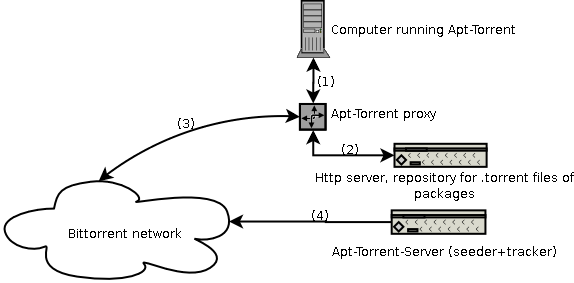
\includegraphics[width=15cm]{image200701/apt-torrent00.png}

簡単な流れは以下のようになります。
\begin{enumerate}
	\item クライアントで \texttt{apt-get update} を行います。

		行うと、\texttt{apt-torrent-proxy}を介して、通信を行います。

	\item \texttt{apt-torrent-proxy} を介して \texttt{apt-torrent} 用の http server と通信します。

		通信を行い、\texttt{/etc/apt/sources.list}に指定してある apt-line のサーバーから情報を取得を試みます。
	\item bittorrent 網 にアクセスします。
	
	\item \texttt{apt-torrent} server から一覧を取得します。

		\texttt{apt-torrent} は seeder\footnote{対象ファイルのデータを全て持っているピア} と 
		tracker\footnote{bittorrentファイルを管理するサーバー}を行っている \texttt{apt-torrent} にアクセスします。
	
	\item \texttt{apt-get install xxxxxxxx} を行います
		\texttt{apt-torrent-proxy} を介して、seeder からデータの取得を試みます。
		取得したデータは Debian Package なので aptが後は勝手に処理をします。
 	
\end{enumerate}

\texttt{apt-torrent} 用 http server を介して bittorrent 網にアクセスしているので、httpで公開されている apt-line から
パッケージを取得しているのと変わらない動きをします。

\subsection{apt との比較}
	今では、apt-get 時に http / ftpサーバーに負荷が集中していますが、\texttt{apt-torrent} を使用することによって
	ひとつのパッケージを ピア同士で共有することが可能になります。\texttt{apt-torrnet} は http / ftpサーバーに
	負荷がかからなくなるひとつの方法になるのではないかと個人的に考えています。
	変化が激しい unstable / testing は無理としても、stable のパッケージを \texttt{apt-torrent} で頒布するのはいい方法
	だと思います。今後、開発者と連絡を取り合い、自宅でも \texttt{apt-torrent} serverを立てて、実験してみようと模索し
	ているところです。
	
\subsection{その他}
 同じような機能を持った Winny のプロトコルを使い、\texttt{apt-winny}を実装してみると面白いと思いました。
 2ch で winny の Linux版である Linny を開発しているようなので(コードはまだない。)期待したいと思います。


\dancersection{プロジェクトトラッカーの勧め}{矢吹 幸治}

\subsection{プロジェクトトラッカーとは何か}
プロジェクトトラッカーは、ある作業にかかった時間を記録するためのプログラムです。
\subsection{なぜトラッカーを使うのか}
このツールは、作業時間を計測するツールです。このトラッカーを使うことにより、

\begin{enumerate}
 \item 自分の能力を高める。
 \item ある作業を開始して完了するまでの時間を予想しやすくする。
 \item 自分の時間の使い方を見直すことができる。
\end{enumerate}

という利点があります。
欠点としては、自分の作業を{\large 記録するのがめんどくさい }という点があ
ります。{\large し
かし記録する利点に比べれば、かける手間は引き合います。}

また、他人に私を観察してもらうよりは、自分で私を観察するほうが、己の自尊
心のために安全です。--- 「他人に指摘してもらう」ことは多くの人にとって苦
痛で、受け入れ難い事です。

\subsection{Debian 4.0(“Etch”)で利用できるトラッカー(Tracker)は?}
以下のパッケージを利用することができます。

\begin{itemize}
 \item  gnotime -- GTK ベース
 \item  karm -- Qt ベース
 \item  wmwork -- X ベース
 \item  worklog -- CUIベース
\end{itemize}

\subsubsection{gnotime}
\begin{wrapfigure}{r}{5cm}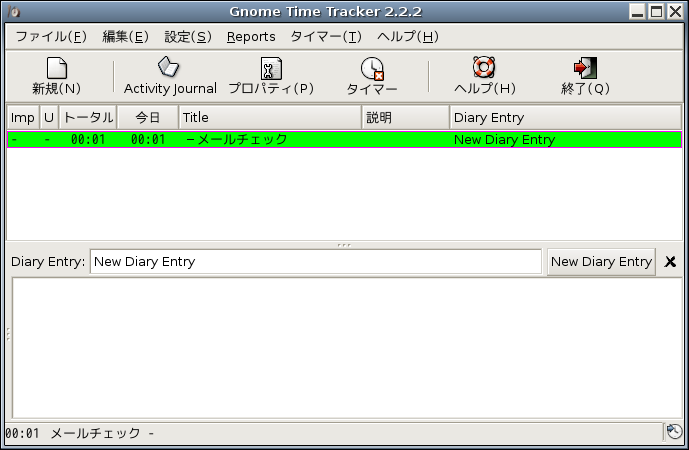
\includegraphics[width=5cm]{image200704/gnotime.png}\end{wrapfigure}
GTKで書かれた、GNOMEと親和性の高いプロジェクトトラッカーです。
日本語も使えて、活動履歴(Activity Journal)も出力できます。DesktopでGNOMEを使っているなら、お勧めです。

\subsubsection{karm}
Qtで書かれたプロジェクトトラッカーです。たぶん便利だと思います。
今回は時間切れで試すことができませんでした。私はKDE使いじゃないので、
誰か小ネタでいいので発表で使い勝手レポートをしてくれるとうれしいです。

\subsubsection{wmwork}

Xがあれば動く、プロジェクトトラッカーです。

\begin{wrapfigure}{r}{2cm}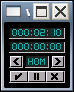
\includegraphics[width=2cm]{image200704/wmwork.png}\end{wrapfigure}

インストール方法は、

\begin{commandline}
 aptitude install wmwork
\end{commandline}

Small is beautiful。
シンプルで Windowmaker や blackbox などのシンプルな window manager と相性が良さそうです。

設定は、wmworkが起動していないときに、~/.wmwork/wmworklogを編集します。
詳細は、/usr/share/doc/wmwork/配下のドキュメントを参照してください。
以下は、/usr/share/doc/wmwork/exsample/worklogを引用しました。

\begin{commandline}
 1# sample wmwork configuration file
 2# do not edit while wmwork is running
 3#
 4# you may save this file as an initial ~/.wmwork/worklog
 5
 6A02:0:comment here
 7PSI:0
 8TEST:0:only 'TES' will be shown
\end{commandline}

上記の設定ファイルをみるとわかりますが、最初の 3 letter がwmworkの表示に使われます。
識別子なのかもしれません。
また、この最初の部分に指定したファイル名でログが取られます。
次に費した時間(秒単位)、最後にコメントという順です。

\verb!~/.wmwork/!以下にロックファイルが作成され、2重起動ができないようになっています。

\subsubsection{worklog}

\begin{wrapfigure}{r}{7cm}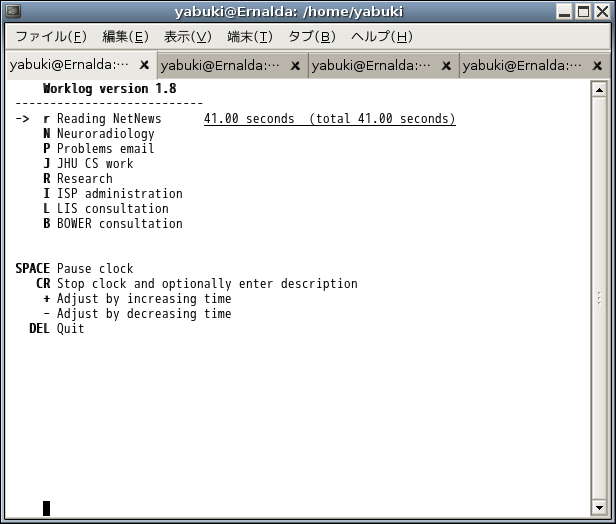
\includegraphics[width=7cm]{image200704/worklog.png}\end{wrapfigure}

CUIで動かすことができます。
sshなどでサーバに入って作業をする場合に便利かもしれません。

\begin{commandline}
 aptitude install worklog
\end{commandline}

このプログラムには、起動するまでに設定ファイルを作成しておく必要があります。
詳しくは、/usr/share/doc/worklog/のファイル群を読んでください。
設定ファイルの書式は、

\begin{commandline}
 キー:割り当てる名前
\end{commandline}

です。例えば

\begin{commandline}
 B:BOWER consultation
 L:LIS consultation
 R:Research
 r:Read NetNews
\end{commandline}

であれば、B,L,R,rのキーで対象となる時間を切替えながら計測できます。残念
ながら表示には日本語(UTF-8)は通りません。(ログには日本語(UTF-8)がそのま
ま出ているのでlvなどでは読むことができました。

{\texttt /usr/share/doc/worklog/examples/projects}に
雛型ファイルがあるので、これをコピーして改変して使うのがよいでしょう。

\begin{commandline}
 alias wl='worklog $HOME/logs/worklog.projects $HOME/logs/worklog.time.log'
\end{commandline}

がお薦めのaliasだそうです。確かに、設定ファイルのキーバインド毎にログが
生成されるので、ディレクトリを作っておくのが良いでしょう。

\dancersection{サーバをエッチにしてみました}{小室 文}

\subsection{intro}
エッチがリリースされてから早一ヵ月たちました。
debian-users mlでは助けを求める亡者の投稿でMLはかつて無い程の盛り上がりを見せていました(います?現在進行形?)。
woodyからsargeへのアップグレード時の盛り上がりを知らないのであれですが、初めてのリリースにちょっとした祭を感じました。
と言う訳でちょうどGWだったので、サーバ2台をsargeからエッチにアップグレードしてみました。

\subsection{やること〜リリースノートを読んでみる〜}
GW前後に日本語のリリースノートが出たので、読んでみました。\\
Debian GNU/Linux 4.0 -- リリースノート\\
\url{http://www.debian.org/releases/stable/releasenotes}

\subsubsection{リリースノートのポイント}
\begin{enumerate}
\item データや設定情報のバックアップを取り、パッケージ状態のチェック (hold状態の物は解決をしておく)
\item sargeで最新状態にする

\item エッチでupdate とupgrade
\item いろいろパッケージをいれる

\item dist-upgrade
\item 最終チェック・再起動・動作確認
\end{enumerate}
\subsubsection {エッチの事(個人的に)}
\begin{itemize}
\item 全体のパッケージ数 18200〜 / エッチでの新しいパッケージ 6500〜 / sargeから約65%のパッケージが更新された
\item default encoding がUTF-8に
\item installerが結構変わったらしい
\item debian-volatile公式リリース
\item Exim4.5からExim4.63に/ Apache2からApache2.2に / PHP5 / Bind9からBind9.3に
\end{itemize}
\subsection{やってみた}
\begin{enumerate}
\item バックアップを取る\\
/etc/以下、/var/lib/dpkgの中身、dpkg --get-selection '*'の出力、/var/backupsなど。後あまり影響はないが/home/以下の隠れファイルとかもXなど使用している場合はバックアップ対象としていたほうがよい
\item パッケージ状態のチェック & セッションの記録
\item (sargeでの)パッケージの更新 \\
/etc/apt/source.listはsargeのままで aptitude update\\
更新候補:libapache-mod-php4 libapache2-mod-php4 libc6 libkrb53 libmagic1 locales man-db php4 php4-comm
\item (エッチでの)パッケージ情報の更新
/etc/apt/source.listをエッチ(stable)にして\\
aptitude update\\
aptitude upgrade\\
削除されたパッケージ:libruby1.6 ruby1.6
\item パッケージの確認・インストール

\begin{enumerate}
\item aptitude install initrd-tools (すでに入っている場合もある)\\
新規に入ったパッケージ:libdevmapper1.02 libselinux1 libsepol1 tzdata\\
削除されたパッケージ:base-config
\item デスクトップ環境があれば\\
aptitude install libfam0 xlibmesa-glu x11-common(入っていたら)\\
新規に入るパッケージ:libfontenc1 libfs6 libx11-data libxau6 libxdmcp6 libxfont1 xbitmaps xcursor-themes xfonts-encodings xfonts-utils xutils-dev\\
削除されたパッケージ:xfree86-common
\item カーネルのアップグレード\\
aptitude install linux-image-2.6-◎◎(すでに2.6系であれば今すぐに更新をする必要は無い)
\end{enumerate}
\item aptitude dist-upgrade\\
アップグレード中に(主にExim4とApache2設定ファイル)各種変更部分の選択を迫られる\\
使われてないから削除されたパッケージ: libfam0c102 libreadline4 ntp ntp-simple\\
新規インストールされたパッケージ:apache2.2-common courier-authlib courier-authlib-userdb cpp-4.1 debian-archive-keyring dmidecode gnupg gpgv laptop-detect libapr1 libaprutil1 libbind9-0 libdb4.3 libdb4.4 libdns22 libedit2 libfribidi0 libgnutls13 libisc11 libisccfg1 libltdl3 liblwres9 libncursesw5 libnewt0.52 libpcap0.8 libpci2 libpq4 libreadline5 libsigc++-2.0-0c2a libslang2 libsp1c2 libsqlite3-0 libssl0.9.8 libtasn1-3 mktemp modconf openbsd-inetd openssh-client openssh-server readline-common sysvinit-utils tasksel-data update-inetd\\
削除されたパッケージ:libnewt0.51 libsp1 netkit-inetd ntp-server apache2-common {\bf exim4-daemon-heavy}\\

\item 確認・再起動
\begin{itemize}
\item /proc/mounts に 'devfs'があればdevfs スタイルのデバイス名の変更をする。
\item liloをブートローダーとして使用している場合、もう一度実行させておく \\
 {/}etc/kernel-img.conf の内容を調べ、do\_{ }bootloader = Yes と書かれていることを確認
\item grubの場合、/etc/kernel-img.conf を編集、update-grub=/sbin/update-grub を/usr/sbin/update-grub に変更する
\end{itemize}
\end{enumerate}

\subsection{怒られた!}
以下のパッケージの処理中にエラーが発生しました: \\
exim4-config postgresql-7.4 postgresql-contrib-7.4 tcsh-kanji postgresql exim4-base postgresql-contrib exim4-daemon-heavy mailagent at exim4 qpopper amavisd-new mutt spamassassin 

怒られた原因と解決方法
\begin{itemize}
\item debconf: unable to initialize frontend: Gnome\\
dpkg-reconfigure debconf にして設定を Dialog に変更。なぜ gnome を選ん
      だのかは自分でも不明です。

\item tcsh conflicts with tcsh-kanji \\
 tcsh-kanji: Depends: tcsh ($\geq $ 6.14.00-6) but it is not installable\\
一番分からずはまった。tcsh-kanji depends on tcshだと思い込んだのとちゃんとエラーを読んでいなかったのが原因。\\
aptitude show tcsh\\
パッケージ: tcsh \\
バージョン: 6.14.00-7 \\
依存: libc6 ($\geq $ 2.3.6-6), libncurses5 ($\geq $ 5.4-5) \\
{\bf 競合: tcsh-kanji (< 6.14.00-6)}\\
置換: tcsh-kanji ( < 6.14.00-6) \\
提供: c-shell, tcsh-kanji\\
上記を見る限りtcshとtcsh-kanjiがconflictsしているようなので、tcsh-kanjiをremove/purgeする

\item /etc/exim4/update-exim4.conf.conf: line 32: acl_check_helo:: command not found \\
昔追加した文を削除してupdate-config.confをして/etc/init.d/exim4 reloadをする(今は使ってないはず)
\item Errors were encountered while processing: exim4-config\\
dpkg -l exim4-configでは Failed-configになっているのでdpkg --configure exim4-configをする

\item exim4-daemon-heavyが exim4-daemon-lightにreplace\\
exim4-daemon-heavyが入っているサーバをアップグレードしたらheavyからlightに置き換わりました。なぜ。

以下の新しいパッケージがインストールされます:\\
  apache2.2-common courier-authlib courier-authlib-userdb cpp-4.1
  debian-archive-keyring dmidecode {\bf exim4-daemon-light} gnupg gpgv
  laptop-detect libapr1 libaprutil1 libbind9-0 libdb4.3 libdb4.4 libdns22
  libedit2 libfribidi0 libgnutls13 libisc11 libisccfg1 libltdl3 liblwres9
  libncursesw5 libnewt0.52 libpcap0.8 libpci2 libpq4 libreadline5
  libsigc++-2.0-0c2a libslang2 libsp1c2 libsqlite3-0 libssl0.9.8 libtasn1-3
  mktemp modconf openbsd-inetd openssh-client openssh-server
  readline-common sysvinit-utils tasksel-data update-inetd\\
以下のパッケージが削除されます:\\
  apache2-common {\bf exim4-daemon-heavy} libnewt0.51 libsp1 netkit-inetd
  ntp-server
\end{itemize}
\subsection{ついで:エッチをstableにした}

もともとtestingの時からetchにしていたPCの/etc/apt/source.listをtestingから stableに直してaptitude updateしたらこんなエラーがでました。

\begin{commandline}
パッケージリストを読み込んでいます... 完了
W: GPG error: http://security.debian.org stable/updates Release:
公開鍵を利用できないため、以下 の署名は検証できませんでした: 
NO PUBKEY A70DAF536070D3A1
W: GPG error: http://cdn.debian.or.jp stable Release: 
公開鍵を利用できないため、以下の署名は検 証できませんでした:
NO PUBKEY A70DAF536070D3A1 NO PUBKEY B5D0C804ADB11277
W: これらの問題を解決するためには apt-get update を実行する必要があるかもしれません
\end{commandline}


なので

\begin{commandline}
gpg  --keyserver wwwkeys.eu.pgp.net --recv-keys A70DAF536070D3A1
gpg --keyserver wwwkeys.eu.pgp.net --recv-keys B5D0C804ADB11277
gpg --armor --export A70DAF536070D3A1 | apt-key add -
gpg --armor --export B5D0C804ADB11277 | apt-key add -
\end{commandline}

とするとエラーが出なくなりました。/etc/apt/source.listで指定している名前が違う=パッケージも違う?のでしょうか。

\subsection{まとめ}
エッチにアップグレードはそんなに難しくない、という事で。
リリースノートとaptitude show パッケージ名があれば大方のトラブルには対応出来るかと思います。

\dancersection{最近 pbuilder ってどうよ?}{上川 純一}

この文書は pbuilder とは何か、そして、最近は何がおきたのか、そしてこれか
ら近い将来になにがおきることが予測されるのかということを紹介する記事です。

Debconf7で紹介する予定の内容です。

\subsection{pbuilder の利用コンセプト}

pbuilder は chroot 内部で利用するベースファイルシステムイメージを管理し、
ビルドのたびに新しいベースファイルシステムイメージを展開することを通して、
クリーンルーム環境でDebianパッケージの試験をするのを簡便にします。

基本操作のためのコマンドがいくつかあります。\texttt{pbuilder create}、 
\texttt{pbuilder update}、 \texttt{pbuilder build}\footnote{pdebuild命令
のほうが便利な場合があります}命令がよく利用される例です。詳細な情報が必
要であれば、 pbuilder のマニュアルを参照してください。
\url{/usr/share/doc/pbuilder/pbuilder-doc.html}にあります。

設定が適切に行われ初期化が終了していれば、\texttt{pbuilder build} コマン
ドは\texttt{.dsc} ファイル(Debianのソースパッケージ)をあたえられると 
chroot 内部でパッケージをビルドします。

\begin{table}[h]
\caption{コマンドの意味}
 \begin{tabular}{|l|l|l|}
 \hline
 操作 & 操作頻度 & 意味 \\
 \hline
 create & 最初に base.tgz を作成するときに一度 & ベースファイルシステムの作成 \\
 update & 一日二回 (unstable のアップデートに伴う) & ベースファイルシステ
 ムの更新 \\
 build & パッケージビルドのたび & Debianパッケージを chroot 内部でビルド
 する \\
 \hline
 \end{tabular}
\end{table}

Debian Developer の通常のある一日に発生するイベントを検討してみましょう。

\begin{center}
 \includegraphics[width=0.5\hsize]{image200705/develcycle.eps}
\end{center}

pbuilder はパッケージのビルドのプロセスの一部、「確認プロセス」に組み込
まれています。\footnote{これは作業フローの一例で、全員がこういう作業フロー
になっているというわけではありません。例えば、一部の開発者はローカルでビ
ルドするということをせず、chroot 内部で全部の作業を完結している場合もあ
り、その場合はローカル環境でのビルドとテストのステップが省略されます。利
点の一つとしてはローカル環境に sid の環境をもたなくてすむことがあげられ
ますが、その点については sid を自分自身でも利用しないことになるため、賛
否両論です。} これは、Build-Dependsを正しく設定できているのか試験するの
に便利です。また簡単な回帰テストのフレームワークとして活用できます。

\subsection{pbuilder 自身の開発の仕組み}

pbuilder 自身がどう開発されているのか解説します。現在、 alioth で提供さ
れているリソースを活用して co-maintain(共同メンテナンス) されています。
最近の主要な開発メンバーは Lo\"ic Minier と上川です。
たまに Matt Kraai と Mattia Dongiliがコミットします。

プロジェクトページは\url{http://alioth.debian.org/projects/pbuilder}にあ
り、ホームページは\url{http://pbuilder.alioth.debian.org/} にあります。
ホームページはpbuilderマニュアルになっています。

ソースコードの管理にはgitを利用しています。レポジトリは下記のコマンドの
いずれかを利用してチェックアウトできます。\footnote{sshアクセスには 
alioth のアカウントが必要です}

\begin{verbatim}
git-clone git://git.debian.org/git/pbuilder/pbuilder.git
git-clone http://git.debian.org/git/pbuilder/pbuilder.git
git-clone ssh://git.debian.org/git/pbuilder/pbuilder.git
\end{verbatim}

\subsection{派生物とその状況}

pbuilder にはいくつかの派生物があり、異なるバックエンドをサポートしてい
ます。それらは別の方法をクリーンルーム試験環境を提供するのに利用していま
す。それらを簡単に紹介します。

\subsubsection{LVM スナップショット版}

誰かが LVM スナップショットをbase.tgz の管理用に利用する仕組みを提案しまし
た。どっかにメールで投稿されています。ただ、誰も採用して開発を継続しよう
とはしていないようです。環境の分離方法は chroot を利用しています。LVM ス
ナップショットの利点としては、 tar アーカイブの展開より格段に高速だとい
う点があげられます。

\subsubsection{user-mode-linux 版}

pbuilder-uml が存在します。どうやらほとんどの人が利用できているようです。
Mattia Dongili たちがこの移植版の開発に携わっています。

base.tgz の展開のかわりに UML cow デバイスでクリーンルーム環境の維持が実
現されています。また、 chroot のかわりに user-mode-linux を活用しており、
結果として各種システムコールが遅くなり全体としては実行オーバヘッドがあり
ます。

\subsubsection{cowdancer 版}

上川が cowdancer 版の作業を 2005 年くらいから行っています。安定している
ようです。base.tgz の展開が\texttt{cp -la } におきかわっており、高速です。

ただし、 cowdancer が libc のコールをフックして実現しているため、一部の
パッケージのビルドに影響が出る可能性があります。\footnote{Etchのリリース
の際には、残念ながら Bug 413912 のような問題が発生しました。}

\subsubsection{qemu 版}

上川が qemu/kqemu/kvm 版の開発を2007年初頭から始めました。QEMUの COW ブ
ロックデバイス機能を活用しているため、base.tgzの展開が不要になります。

qemu版は別アーキテクチャ向けのビルド(クロスビルド)機能を提供するという特
徴があります。たとえば i386 マシン上でARM用のパッケージをビルドすること
だってできるはずです。

\subsection{さらなる開発のアイデア}

\subsubsection{インストールテスト}

インストールテストについては、いくつかの piuparts のようなプロジェクトが
あり、pbuilder でも応用できそうです。コンセプトを実装する簡単な例として
のスクリプトは pbuilder で提供しています。
\url{/usr/share/doc/pbuilder/examples/execute_installtest.sh} です。

\begin{verbatim}
pbuilder execute \
  /usr/share/doc/pbuilder/examples/execute_installtest.sh \
  pbuilder
\end{verbatim}

このコマンドは 指定したパッケージを chroot 内部で apt-get でインストー
ルしようとし、成功するかしないかを確認してくれます。

\subsubsection{パッケージのテスト}

パッケージのテストの機能は重要です。とくに、開発者の時間は限られており、
手動でテストを繰り返すというのは楽しいことではないからです。pbuilder は
例としてフックスクリプトを提供しています。
\url{/usr/share/doc/pbuilder/examples/B92test-pkg} はパッケージのビルド
が成功した場合に、テストを実行するようになっています。

テストファイルは\verb!debian/pbuilder-test/NN_name! (NN は数字です)にお
きます。ファイル名は run-parts の標準に従います。\footnote{ファイル名に 
'.' が入っていたら無視されますよ!}.

\subsubsection{aptitude}

pbuilder は現在 apt-get コマンドを活用しています。しかしながら、 
aptitude の普及に伴い、aptitude を活用する方法を考える時期にきているかも
しれません。

\subsubsection{apt-key support}

pbuilder はあいかわらず apt-key をサポートしていません。現在の stable リ
リースで apt-key が提供されているため、そろそろ apt-key をサポートしよう
かな。

\subsubsection{build-dependency parser}

Build-Depends を解析するパーサは古く、最適ではありません。それをうけて、
Lo\"ic Minier はいくつかの再実装を試行しています。

\subsubsection{buildd.net のような仕組みのサポート}

pbuilder はたくさんのログを提供するのですが、pbuilder 自体は歴史の概念を
もちあわせていません。pbuilder 単体ではログを集めて活用するというように
はなっていません。\footnote{\texttt{pbuildd}を作成するというプロジェクト
は存在しました。最近どうなってるのかについては把握していません。} 過去の
ビルドログをローカルに集めて、各ビルド間での差分を確認することを通して、
問題を検出できるかもしれません。debdiff などのツールと組み合わせて利用す
るとよいかもしれませんね。


\subsection{References}

\begin{itemize}
 \item \url{http://pbuilder.alioth.debian.org/} か
 \url{/usr/share/doc/pbuilder/pbuilder-doc.html}: pbuilderマニュアル
 \item cowdancer パッケージ
 \item piuparts パッケージ
 \item autodebtest: Ubuntu の自動テストシステム
 \item schroot / dchroot 
 \item buildd
\end{itemize}

\dancersection{Debian on SuperH}{岩松 信洋}
\label{debiansuperh}

今年に入って、ちまちまと Debian の SHへのポーティング を再始動したのですが、
Debconf7 の BOF で Debian porting for SH が通ってしまいました。
Debconf7 で発表する内容を以下にまとめたいと思います。

\subsection{SuperH とは}

SuperH( 以下、SH ) は ルネサステクノロジ\url{http://www.renesas.com/}が販売している 組込み向けの CPU です。
特徴としては以下のものがあります。
\begin{itemize}
	\item 日本国産
	\item 低電圧
	\item 種類が多い

		SH1/SH2/SH2A/SH3/SH3-DSP/SH4/SH4A/SH4AL/SH4AL-DSP ......
\end{itemize}

携帯電話、HDD コンポ、 液晶テレビ、カーナビゲーションシステム等で採用され、Linux が動作しています。

\subsection{歴史}

2000年前後から Debian に SuperH を移植しようとする活動が行われてきました。
それらを紹介します。

\subsubsection{第 0 次 SHブーム}
約 7 年前、情報処理推進機機構 (旧 情報処理振興事業協会)、\footnote{英語名 Information-technology Promotion Agency} 略称「IPA」
の未踏ソフトウェア創造事業に採択され、SHが Linux に移植されました。
\footnote{http://www.ipa.go.jp/NBP/12nendo/12mito/mdata/5-9gh/5-9gh.pdf}
\footnote{http://lc.linux.or.jp/lc2001/papers/linux-superh-paper.pdf}

そして、この時の移植チームのメンバの一人で、Debian Developer である八重樫 剛史 氏\footnote{yaegashi@debian.org}を中心に、X Hacker
である石川 睦氏\footnote{ishikawa@debian.org}が Debian に移植を試みました。
このときの状況は、

\begin{itemize}
 \item サポートアーキテクチャは sh( little endian ) と sheb( big endian )
 \item baseはできており、コンパイラも当時最新のもの
 \item ネイティブで作成するのはリソースが足りないため、DODES プロジェクトを立ち上げ、コンパイル
\end{itemize}

とすばらしいものでした。

過去に行われた Debian Conference 2001 Tokyo, Japan \footnote{http://www.debian.or.jp/community/events/2001/1025-dcj2001/}
で石川氏 が Debian GNU Linux on SuperH \footnote{ http://www.debian.or.jp/community/events/2001/1025-dcj2001/HANZUBON-debian-sh.html} として発表されておられます。


% http://lists.debian.org/debian-devel/2001/03/msg01188.html

しかし、八重樫氏が Debian-superh ML に移植を行う旨

\url{http://lists.debian.org/debian-superh/2001/12/msg00013.html}

を伝えたところ、

\begin{itemize}
	\item big endian 必要ないのでは?
	
		\url{http://lists.debian.org/debian-superh/2001/12/msg00014.html}
		
%	\item サポートアーキテクチャは sh3/sh4( little endian ) と sh3eb/sh4eb( big endian )にすべきだ。
%	
%		\url{http://lists.debian.org/debian-superh/2001/12/msg00013.html}

	\item SH3/SH3eb , SH4/SH4eb の4つのアーキテクチャを入れると、サーバーの容量の問題が発生するため、
		入れること難しいと思う。
		
		\url{http://lists.debian.org/debian-superh/2001/12/msg00020.html}

\end{itemize}
という問題提議があり、sh3/sh3eb/sh4/sh4eb にアーキテクチャを分けたまま、移植は止まってしまったのでした。
\url{http://lists.debian.or.jp/debian-devel/200011/msg00044.html}

当時、ビルドに使われていたマシン以下の通りです。

% Hitach UL Solution Engine
\begin{figure}[htbp]
 \begin{minipage}{0.5\hsize}
  \begin{center}
   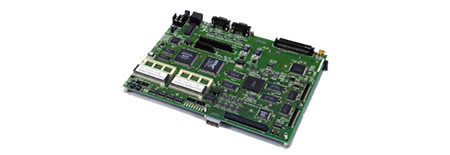
\includegraphics[width=0.7\hsize]{image200705/solutionengine.jpg}
  \end{center}
  \caption{Solution Engine}
 \end{minipage}
 \begin{minipage}{0.5\hsize}
  \begin{tabular}{|l|l|} \hline
   & Solution Engine \\ \hline
   CPU & SH7709 ( 133Mhz ) \\ \hline
   memory & 32MB\\ \hline
   Flash & 4MB \\ \hline 
   IDE  & PCMCIA slot \\ \hline
   Ethernet & stnic \\ \hline
  \end{tabular}
 \end{minipage}
\end{figure}

% CAT
\begin{figure}[htbp]
 \begin{minipage}{0.5\hsize}
  \begin{center}
   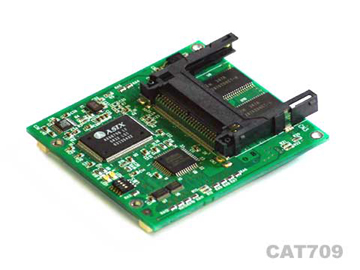
\includegraphics[width=0.6\hsize]{image200705/cat709.jpg}
  \end{center}
  \caption{CAT 709}
 \end{minipage}
 \begin{minipage}{0.5\hsize}
  \begin{tabular}{|l|l|} \hline
   & Solution Engine \\ \hline
   CPU & SH7709 ( 133Mhz ) \\ \hline
   memory & 32MB\\ \hline
   Flash & 8MB \\ \hline 
   IDE slot & CF Slot \\ \hline
   Ethernet & なし\\ \hline
  \end{tabular}
 \end{minipage}
\end{figure}

% Jornada 6xx
その他に Hewlett-Packard 社から販売されていた、Jornada6xx シリーズも使われていたとのこと。

%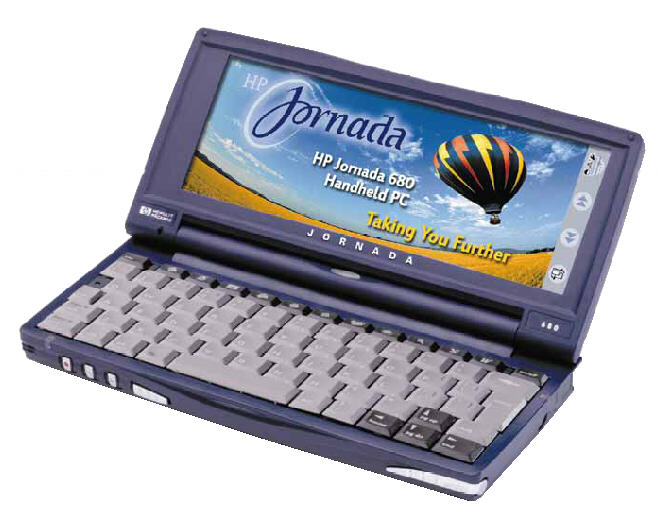
\includegraphics[width=0.2\hsize]{image200705/jornada680.jpg}

\subsubsection{第 1 次 SHブーム}

約2年前、SH を採用した NAS 、LANDISK / LANTANK  が I/Oデータさんから販売されました。
これらは I/O データさんに在籍しておられる、kinneko さん \footnote{http://d.hatena.ne.jp/kinneko/} および iohack project \url{http://iohack.sourceforge.net}
の元、開発が行われ Debian パッケージでシステムが構築されていました。
安値であり、自由に触ることができるということで、人気があり、各 Linux 雑誌でも取り扱われ、ブームを築きました。
これが 第 1 次 SH ブームです。

以下に LANDISK / LANTANK のスペックを示します。
\begin{figure}[htbp]
 \begin{minipage}{0.5\hsize}
  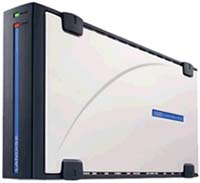
\includegraphics[width=0.6\hsize]{image200705/landisk00.jpg}
  \caption{LANDISK}
 \end{minipage}
 \begin{minipage}{0.5\hsize}
  \begin{tabular}{|l|l|} \hline
   & LANDISK \\ \hline
   CPU & SH7751R ( 266Mhz ) \\ \hline
   SDRAM & 64MB\\ \hline
   Flash & ROM \\ \hline
   IDE & UDMA133 PATA (ACARD ATP865)\\ \hline
   Ethernet & 10/100Base-T (RTL8139CL + EEPROM 93C46) \\ \hline
   USB & USB2.0 TypeA Conn x2 (NEC D720101GJ) \\ \hline
   値段 & 約35000円 \\ \hline 
 \end{tabular}
 \end{minipage}
\end{figure}


\begin{figure}[htbp]
 \begin{minipage}{0.5\hsize}
  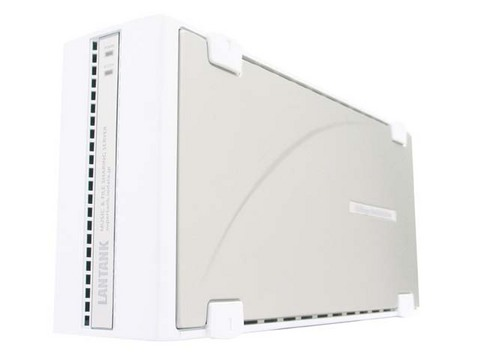
\includegraphics[width=0.9\hsize]{image200705/lantank00.jpg}
  \caption{LANTANK}
 \end{minipage}
 \begin{minipage}{0.5\hsize}
  \begin{tabular}{|l|l|} \hline
   & LANTANK \\ \hline
   CPU & SH7751R ( 266Mhz ) \\ \hline
   SDRAM & 64MB\\ \hline
   Flash & ROM \\ \hline
   IDE & UDMA133 PATA (ACARD ATP865) 2disk support  \\ \hline
   Ethernet & 10/100Base-T (RTL8139CL + EEPROM 93C46) \\ \hline
   USB & USB2.0 TypeA Conn x2 (NEC D720101GJ) \\ \hline
   値段 & 約19800円 \\ \hline
  \end{tabular}
 \end{minipage}
\end{figure}

しかし、SH の販売元であるルネサステクノロジはこのブームをうまく活用することができず、
そのまま消えていこうとしていたのでした。

\subsubsection{歴史は繰り返さないために}
終了してしまったように見えた、 SH の Debian への移植ですが、
私がパッケージを再ビルドし、再移植を行うことにしました。
理由としては、
\begin{itemize}
 \item SH で 容易に使用できるディストリビューションがない。
 
       gentoo でサポートされているが、ビルドが面倒。
 
 \item 仕事でも使えるようにしたい :)
       
	個人的理由。

 \item Debian User だから。
 
\end{itemize}

私は今回の移植では、以下のポリシーで作成することにしました。

\begin{itemize}
 \item Debian でサポートするアーキテクチャ

   SH4のみをサポートします。
   SH4A 等もすべてSH4として扱います。
   
 \item SH3 サポート
 
   SH3 と SH4 の大きな違いは FPU があるか、ないか です。
   SH3 は SH の Linux カーネルでサポートされた math-emu を使って、math をエミュレーションする方法を取ります。
   もちろん、math-emuを使うと、遅くなりますが、SH3 を採用した CPU がほとんど存在しないため、
   コストにはならないと考えています。
   
   他には、cache の違いもあるので、これをうまくトラップできる仕組みを入れる必要があります。
   
 \item big endian サポート
 
   big endian もサポートするすることも考えています。
   
\end{itemize} 

\subsection{現状}

\subsubsection{開発メンバー}
現在、基本的に開発を一人でやっていますが、以下の方々にサポートをしてもらっています。

\begin{itemize}

	\item 小島先生
		binutils SH メンテナ
		
		SH の分からないところは質問させていただいています。

	\item 武藤さん
	
		buildd の構築で相談に乗ってもらっています。

	\item kinnneko さん
	
		いろいろ手伝ってもらっています。

	\item gotom さん
	
		Debian glibc メンテナ.
		開発用のボードは渡したんだけど.....。

	\item 上川さん
	
		LANTANK買わせたんですが.....。
\end{itemize}

\newpage

\subsubsection{現在使用しているビルドマシン}

現在、ビルドに使用しているマシンは以下の通りです。

\begin{enumerate}

\item LANTANK x 3

\begin{figure}[htbp]
  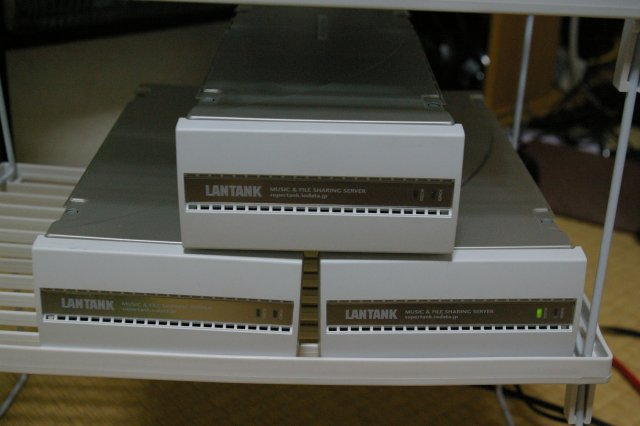
\includegraphics[width=0.8\hsize]{image200705/lantank01.jpg}
  \caption{LANTANK x 3} 
\end{figure}

\item RTS7751R2D

\begin{figure}[htbp]
 \begin{minipage}{0.5\hsize}
  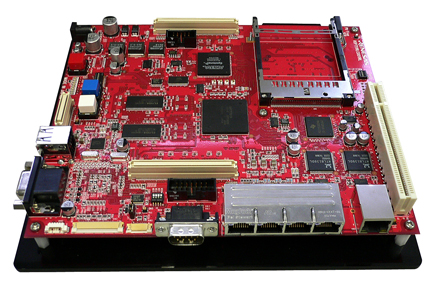
\includegraphics[width=0.9\hsize]{image200705/r2d.jpg}
  \caption{RTS7751R2D}
 \end{minipage}
 \begin{minipage}{0.5\hsize}
  \begin{tabular}{|l|l|} \hline
   & RTS7751R2D \\ \hline
   CPU & SH7751R ( 266Mhz ) \\ \hline
   SDRAM & 64MB\\ \hline
   Flash & ROM \\ \hline
   IDE & CF slot and  PCMCIA \\ \hline 
   Ethernet & 10/100Base-T (RTL8139CL + EEPROM 93C46) \\ \hline
   USB & SM501 USB1.1 (Silicom Motion) \\ \hline
  \end{tabular}
 \end{minipage}
\end{figure}

ルネサスソリューション様から提供していただきました。
\end{enumerate}

\subsubsection{パッケージ状況}

現在のパッケージ状況は以下の通りです。

\begin{itemize}
	\item SH4のみをサポート
	
		ビッグエンディアンのマシンを持っていないため。

	\item build-essential ビルド完了
	
		gcc-4.1.2 / binutils / glibc-2.5 

	\item sid debootstrap サポート
	
		debootstrap できるパッケージができています。

	\item SH4 buildd 稼働中
	
		公開はされていませんが、SH4 向けの buildd が稼動中です。
		今後、buildd.net \url{www.buildd.net} に登録する予定です。
		
\end{itemize}

これらの成果物を \url{http://www.nigauri.org/~iwamatsu/debian/debian-sh4/}で公開中です。

\subsection{今後の課題}

\begin{itemize}

\item Debian の正式なサポートアーキテクチャにする
\item buildd.net への登録
\item builddのメンテナンスが行える体制を作る

	共同メンテナを募集しています。
\item 回線の保持 

	buildd 用マシンネットワークの確保

\end{itemize}

\subsection{リンク}

\begin{itemize}
    \item SuperH \url{http://www.renesas.com}
    \item IRC \#debian-superh @ oftc.net
    \item ML  debian-superh@lists.debian.org
    \item Debian Packages repository
	\url{http://www.nigauri.org/~iwamatsu/debian/debian-sh4/}

  \item iohack project
	\url{http://iohack.sourceforge.jp}

\end{itemize}


\dancersection{Debian の情報フロー}{上川 純一}
\label{debianinfo}

\begin{minipage}{0.6\hsize}
 Debian etch を活用するためには、何をしたらよいですか?  今日のようにみん
 なあつまって議論すると、いろいろな新しい発見や情報が出てくるけど、それっ
 て普段みんなどうしているの?その疑問を追求するためにワークショップをして
 みました。

 まず建前から確認してみましょう。

 \begin{itemize}
  \item 基本はリリースノート
  \item BTS で生きた情報を得る
  \item debian-users メーリングリスト
 \end{itemize}

しかし実際の運用は少し違うこともあります。理由としては例えば次のようなも
 のがそれぞれあります。

\begin{itemize}
 \item リリースノート: 一度リリースされてしまうとそう簡単に項目が追加さ
       れる類のドキュメントではない。
 \item BTS: 英語なので日本では活用しているメンバーが限られる。また英
       語が問題とならなかったとしても、BTSの仕組みとして、情報がパッケー 
       ジ単位で管理されるため複合的に発生する問題は登録しにくい
\end{itemize}

現状の運用はどうかというと、ワークショップで出てきた話を総合すると、実際
は次のような流れになっているようですね。

 \begin{itemize}
  \item IRCでまずきく
  \item googleで検索 (blog とか スレッドテンプレで発見)
  \item 報告は blog に記述
  \item 2chで質問が出たりしたらblogを参照してスレッドテンプレに登録
 \end{itemize}
\end{minipage}
\begin{minipage}{0.4\hsize}
 \includegraphics[width=0.9\hsize]{image200705/problemcycle.eps}
\end{minipage}

では、現状を把握したところで、この仕組みのままで改善するか、違う仕組みを
考えるか、検討していけばよいはずです。続きはまた。


\dancersection{Debian勉強会資料の作成方法}{上川 純一}
\label{sec:debmtg2006res}

\subsection{レポジトリを取得し、パッケージの準備を行う}

レポジトリをチェックアウトします。

\begin{commandline}
$ cvs -d :ext:cvs.alioth.debian.org:/cvsroot/tokyodebian . 
\end{commandline}

ディレクトリ構成は次のようになっています。

\begin{itemize}
 \item monthly-report: TeXのソースが全部フラットにおいてあります。ファイ
       ル名は、 debianmeetingresumeYYYYMM.texという名前になっています。
       プレゼンテーションファイルは
       debianmeetingresumeYYYYMM-presentation.tex という名前になってい
       ます。
       \begin{itemize}
	\item imageYYYYMM:各月用の画像ファイル
	\item debian: デビアンパッケージ用ディレクトリ
       \end{itemize}
 \item muse: ウェブ(wiki)
 \item meetinglog: 議事録置場
\end{itemize}

ビルドに必要なパッケージをインストールします。

\begin{commandline}
apt-get install ptex-bin dvipdfmx latex-beamer \
 okumura-clsfiles gs-esp xpdf xpdf-japanese 

\end{commandline}

編集に便利なツールもついでにインストールしてみてもよいでしょう。

\begin{commandline}
 apt-get install whizzytex advi emacs21 yatex
\end{commandline}

\subsection{pLaTeXで文書作成}

make コマンド一発で 
PDFファイルまで、コンパイルすることができます。
Makefile には、あらゆる debianmeeting*.texファイルに関して .pdf ファイルを作成するよう
にルールが作成されています。

注意する点として、印刷を考え、ページ数が4の倍数になるようにしてください。

\begin{commandline}
SOURCE:=$(wildcard debianmeeting*.tex)
DVIFILES:=$(SOURCE:%.tex=%.dvi)
PDFFILES:=$(SOURCE:%.tex=%.pdf)
all: $(PDFFILES)

%.pdf: %.dvi
	dvipdfmx $< 

%.dvi: %.tex
	# check kanji-code of the tex file.
	iconv -f iso-2022-jp -t iso-2022-jp < $< > /dev/null
	platex $<
	platex $<
	platex $<

clean:
	-rm *.dvi *.aux *.toc *~ *.log *.waux *.out _whizzy_* *.snm *.nav *.jqz

\end{commandline}


\subsubsection{画像ファイルの処理}

画面写真の画像を追加するときは、できるだけサイズの小さい png などを利用
してください。グラフなどの線画であれば、epsでかまいません。png であれば、 
ebb コマンドを利用してbounding box を作成してください。

\begin{commandline}
 ebb XXX.png
\end{commandline}

ps であれば、 eps2epsでバウンディングボックスを追加してあげるとうまくい
きます。sodipodi の出力する ps を eps2epsで処理すれば sodipodi で画像を
作成することができます。

\subsection{pLaTeX+latex-beamerで文書作成}

残念ながら whizzytex でプリビューはうまく動かないです。

がりがりと作成し、xpdfでプリビューしながらがんばって作成してください。


\subsection*{参考:Debian 勉強会のウェブインタフェース}

Debian 勉強会のウェブインタフェースについて解説します。

初期は
\url{http://www.netfort.gr.jp/~dancer/column/2005-debianmeeting.html.ja} 
にあるページを手動で生成していました。

CMSを採用したいところでしたが、CMSを探索している間中ずっと手動で生成して
いるのも困難なので現状のページにかわりました。
\url{http://tokyodebian.alioth.debian.org/2006-11.html} のようなページに
なっています。

該当するファイルはCVSレポジトリの muse/ ディレクトリにあります。emacs を 
wiki 処理系として利用しており、 Makefile から emacs を呼出し、HTML を静
的に生成するようになっています。

今後実現していきたい内容としては
\begin{itemize}
 \item RSSをはくアナウンスページ
 \item ユーザ参加登録と同時に事前課題登録
 \item 事後のアンケート
 \item 登録ユーザへの次回通知
 \item 事後の資料公開・感想文公開
\end{itemize}

があります。

muse-el は一般的な構成ではなく開発もあまり活発でないので、今後利用ツール
を変更したいと考えています。

\dancersection{Debian勉強会2006年結果統計}{上川 純一}
\label{sec:debmtg2006}

\subsection{Debian勉強会評価項目}

Debian の開発者を増やしていき、Debian の活動を活発にしていきたい、そうい
う思いでDebian 勉強会は開催しています。
そもそも Debianのユーザの裾野がひろがり、活発なユーザが増え、
ユーザが開発者になろう、と思って、NMプロセスを通らないと、Debian Developer は増
えません。

%sodipodi経由、eps2epsで作成
% eps2eps hierarchy.ps hierarchy.eps
\includegraphics[width=0.5\hsize]{image200612/hierarchy.eps}

Debian 勉強会が成功した、という場合、何がおきた場合でしょうか。

\begin{itemize}
 \item 直接貢献: バグがどんどんクローズされていき、新機能が追加
 \item 各種アプリケーションの日本語対応が進捗
 \item 日本から Debian Developer を生み出す
 \item 日本の Debian ユーザが増える
 \item すでに経験の豊富な Debian Developer の知識を展開
 \item ドキュメントが増える
\end{itemize}

直接評価できる指標としては下記があるでしょう。

\begin{itemize}
 \item 日本語で増えたドキュメント数
 \item Debian Developer の参加者数
 \item Debian Developer でない参加者数
 \item 新規の参加者
 \item 新規に参加して二度以上参加してくれた参加者の数
\end{itemize}

それでは、値がどういうものか見てみましょう。

概算の値なので、正確ではありません。過去の記録を発掘して、今後の検討のた
めにひねり出しているものです。

\subsection{新規の参加者}

\begin{itemize}
 \item 2005年1月: 20 人
 \item 2005年2月: 6 人
 \item 2005年のこり: 12 人
 \item 2006年 -6月: 9人
 \item 2006年 -10月: 14人
\end{itemize}

\subsection{新規に参加して二度以上参加してくれた参加者の数}

参加者の統計です。

\begin{itemize}
 \item 2005年: 39人中 21人
 \item 2006年上半期 (-6月): 9人中 5人
 \item 2006年下半期 (-10月): 14人中 2人
\end{itemize}

\subsection{Debian Developer比率}

のべ参加者の中からのおおよその分析ですが、どれくらいの参加者が Debian
Developer で、どれくらいの参加者が New Maintainer Queue に入っているか、
の統計です。

\begin{itemize}
 \item 2005年:39人中 DD 4 人? NM 3 人
 \item 2006年 -10月:36人中 DD 6 人 NM 6 人
\end{itemize}

\subsection{参加人数}

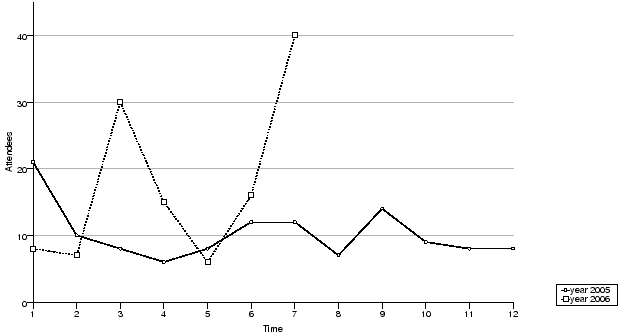
\includegraphics[width=1\hsize]{image200612/people-chart.png}

 
 \begin{table}[ht]
\begin{minipage}{0.6\hsize}
 \caption{参加人数(2006年)}\label{tab:count2006}
 \begin{center}
  \begin{tabular}{|l|c|l|}
 \hline
 & 参加人数 & \\
 \hline
 2006年1月 & 8 & policy,Debian勉強会でやりたいこと\\
 2006年2月 & 7 & policy, multimedia \\
 2006年3月 & 30 & OSC: debian勉強会,sid \\
 2006年4月 & 15 & policy, latex \\
 2006年5月 & 6 & mexico \\
 2006年6月 & 16 & debconf, cowdancer\\
 2006年7月 & 40 & OSC-Do: MacBook Debian \\
 2006年8月 & 17 & 13執念 \\
 2006年9月 & 12 & 翻訳、Debian-specific、oprofile \\
 2006年10月 & 23 & network, i18n会議、Flash、apt \\
 2006年11月 & 20 & 関西: bug, sid, packaging \\
 2006年12月 & 14 & 忘年会 \\
 \hline
  \end{tabular}
 \end{center}
\end{minipage}
\begin{minipage}{0.35\hsize}
 \caption{参加人数(2005年、概算)}\label{tab:count}
 \begin{center}
  \begin{tabular}{|l|c|}
   & 参加人数 \\
 \hline
   2005年1月 & 21 \\
   2005年2月 & 10 \\
   2005年3月 (早朝)& 8\\
   2005年4月 & 6\\
   2005年5月 & 8\\
   2005年6月 & 12\\
   2005年7月 & 12\\
   2005年8月 & 7\\
   2005年9月 & 14\\
   2005年10月 & 9\\
   2005年11月 & 8\\
   2005年12月 & 8 \\
  \end{tabular}
 \end{center}
\end{minipage}
 \end{table}

\subsection{実施テーマ}

今年は下記のテーマを実施しました。
\begin{itemize}
 \item Debian weekly news クイズを隔月で
 \item グループワーク:Debian勉強会でやりたいこと
 \item Debian Policy 入門
 \item Debian Multimedia Project
 \item Debian 勉強会紹介
 \item sid のすすめ
 \item LaTeX 
 \item DebConf2006 報告
 \item cowdancer 
 \item MacBook Debian
 \item module-assistant
 \item oprofile
 \item 翻訳のすすめ
 \item Debian-specific
 \item i18n
 \item Flash
 \item Bug tracking system
 \item Debian packaging.
\end{itemize}

\subsection{会議の構成}

今年のDebian 勉強会にはおおきくわけて三種類の会議形態がありました。

\begin{itemize}
 \item OSC(春、秋)
 \item 出張(OSC北海道、メキシコ、KOF)
 \item 通常
\end{itemize}

東京のOSCでの開催は、通常の勉強会に参加するよりハードルを低く設定してい
ます。できるだけ多くの人たちに参加してもらうことを目的としています。これ
でDebian勉強会の雰囲気をしってもらい、興味を持ってもらい、通常の勉強会に
参加しやすくなるように配慮しています。

Debian 勉強会は、ふたつの目的をもっています。そのふたつの目的にあわせた
会議設定をしています。一つめはDebian 開発者の開拓です。二つ目はDebianユー
ザの集まる場所を提供することです。

OSC, KOF など、年三回程度のイベントにおいては、他の主催者の企画したイベ
ントのうえでイベントを実施しています。コストも、集客方法も主催者側に一任
しています。また、実務上、事前課題の設定などもできていません。

毎月実施している勉強会については、より目的意識の高い会として位置づけてい
ます。Debian 開発の側に参画し、よりドキュメントを生成する側にまわり、み
んなでDebianの現在の課題についてブレーンストーミングできるようになること
が目標です。そのため、事前課題を準備して、目的を共有できるような仕組を準
備しています。

また、現状の勉強会の運営については、毎年一回、12月開催の勉強会に確認し、
来年度の運営方針を確認することにしています。


\dancersection{Debian勉強会2006年、作業フロー}{上川 純一}
\label{sec:debmtg2006flow}

どういう作業をしたでしょうか。書き出してみましょう。

\subsection{年に一回の作業}

\begin{itemize}
 \item 年次計画を仮決め、毎月どの日に開催するのかを決定して、
       それをベースにしてその後の議論をする。
 \item tokyodebian-2006 メーリングリストの作成
\end{itemize}

\subsection{事前準備}

\begin{itemize}
 \item 開催二ヵ月前: 開催場所の予約
 \item 資料の作成
 \item 開催二週間前: \url{http://utage.org/enkai} 宴会君への登録
 \item 開催二週間前: \url{http://tokyodebian.alioth.debian.org/} ウェブサイトの更新
 \item 開催二週間前: mixi と debian-users/debian-devel にアナウンス
 \item 開催二日前:印刷、資料は4の倍数のページ数にして、kinko's にコピー
       依頼。\footnote{2006年10月、ウェブベースで依頼してみたところ無事印刷された
       ので、今後はウェブで依頼する予定。}
 \item 開催一日前:宴会場所の予約
\end{itemize}

\subsection{事後処理}

\begin{itemize}
 \item 議事録の作成
 \item blogトラックバックの収集
\end{itemize}

\dancersection{Debian勉強会 2007年度計画検討結果}{上川 純一}
\label{sec:debmtg2007plandone}

2007 年度の計画を検討した結果次のような内容が出てきました。

Debian が現在市場に提供している付加価値としては下記がある。
\begin{itemize}
 \item 	 デプロイしやすいしくみであること
 \item	 ライセンスが明確であること
 \item	 たくさんソフトウェアがあること
 \item	 アップグレードが平穏であること
 \item	 くだらないパッケージもはいっていること
 \item	 ソースコードが簡単にとってこれること
 \item	 ユーザが多いこと
 \item	 学ぶことがおおいこと
\end{itemize}

また外部的な要因として
\begin{description}
 \item[Windows] VISTA の公開βテスト開始
 \item[Mac OSX] iPhone, Leopard
 \item[他のディストリビューション] FC, SUSE, RHEL の新リリースが出る、Ubuntu も出るが、宇宙に再度いってしまうのではないか?
 \item[ハードウェア] Quad core, Wii/PS3/.. などが出る
 \item[ユーザの期待として] 次はさすがにGUIでD-iできるだろう
\end{description}
というのがある。

ユーザの拡大方向としては、下記の案が出てきた。
\begin{description}
 \item[主婦]
 \item[学生] 教育にDebianを利用するべきだ
\end{description}
また、今年の活動は、来年を考えて動くべきだろう。

以上をふまえての今年度の計画は下記で実施する。
\begin{itemize}
 \item[2] 小林さん幹事
 \item[3] 岩松さん担当でOSC
 \item[4] えとーさんでエッチインストール大会
 \item[5] ごとむさん主催でgoogle開催(!?)
 \item[6] やぶきさんでえじんばら開催
 \item[7] Debconf参加報告会
 \item[8] Debian14周年
 \item[9以降] 後で考える。
\end{itemize}

\newpage
\dancersection{Debian Weekly News trivia quiz}{上川 純一}

ところで、Debian Weekly News (DWN)は読んでいますか?
Debian 界隈でおきていることについて書いているDebian Weekly News。
毎回読んでいるといろいろと分かって来ますが、一人で読んでいても、解説が少
ないので、
意味がわからないところもあるかも知れません。みんなでDWNを読んでみましょう。

漫然と読むだけではおもしろくないので、DWNの記事から出題した以下の質問にこたえてみてください。
後で内容は解説します。



\subsection{2006年41号}
\url{http://www.debian.org/News/weekly/2006/41/}
にある11月28日版です。

\santaku
{Debian Conference 7 日程が決まりました。いつからでしょうか。}
{4/1}
{5/22}
{6/17}
{C}


\santaku
{Debian Project に新しい開発用マシンが導入されました。どのマシンでしょうか。}
{Sun Fire T2000}
{Sony Playstation 3}
{TiVo Series2 DVR}
{A}


\subsection{2006年42号}
\url{http://www.debian.org/News/weekly/2006/42/}
にある2006年12月26日版です。

\santaku
{Linux Conference Australia で開催される Debian 関係のイベントは今回で何回目か}
{1}
{3}
{6}
{C}

\santaku
{最近急上昇してDebian内で3位人気のアーキテクチャになったアーキテクチャは?}
{ARM}
{PPC}
{AMD64}
{A}

\santaku
{etchがフリーズされたのはいつ?}
{11/11}
{12/11}
{12/24}
{B}

\santaku
{Debian のインストール CD イメージはどれくらいの頻度で更新されているか?}
{毎日}
{毎メジャーリリース}
{毎マイナーリリース}
{A}



\subsection{2007年01号}
\url{http://www.debian.org/News/weekly/2007/01/}
にある1月23日版です。

\santaku
{creative commons 2.5 は DFSG互換か?}
{ちがう}
{DFSG互換です}
{むしろGPLとまったく同じ}
{A}

\santaku
{Kenshi Mutoのアナウンスによると、Takeshi Yaegashiは何にDebianをインストールするのに成功した?}
{PLAYSTATION 3}
{Wii}
{XBox 360}
{A}

\santaku
{Florian Lohoffはどんな変化に気付いたか?}
{woodyがミラーから取り除かれた}
{sargeのアーカイブに侵入された形跡がある}
{etchへの開発者の興味が薄れている}
{A}

\santaku
{Joseph Smidtはリリースに関して何を提案したか?}
{unstableとtestingだけをサポートするようにして保守作業を楽にしよう}
{etchはリリースされないまま古くなりつつあるので適当にリリースしてlennyに全力を注ぎ込もう}
{そろそろDebianもXPやVistaといったよくわからない名前をリリースにつけるようにしよう}
{A}

\subsection{2007年02号}
\url{http://www.debian.org/News/weekly/2007/02/}
にある1月30日版です。

\santaku
{Roberto C. Sanchezが提案したのは何か}
{全員が自分の誕生日をDebianとして祝うべきだ}
{Debianのスクリーンショットのレポジトリを準備して、それぞれのパッケージ
に対応させる}
{Debianを全員使うべきだ}
{B}

\santaku
{Robert Millanが作成したwin32用プログラムは?}
{Windows Vistaを自動的にダウンロードし上書きインストールしてくれるインストーラ}
{ユーザの手間を省くために、Outlook Expressのアドレス帳に載っているアドレスをlists.debian.orgのメーリングリストすべてに自動登録してくれるプログラム}
{Debian Installerを自動的にダウンロード・起動してくれるランチャー}
{C}

\santaku
{1月31日に締め切られたのは?}
{第24回東京エリアDebian勉強会のblogでの報告}
{Debian etchベータ版のテスターの募集}
{Debian Conference 7のスポンサー希望者の参加登録}
{C}

\santaku
{Luis Matosがetchのカーネルに関して提案したのは?}
{kvmが利用できるように2.6.20を使おう}
{LinuxではなくkFreeBSDを使おう}
{ハードウェアサポートのためにポイントリリースでカーネルの更新を行おう}
{C}

\subsection{2007年03号}
\url{http://www.debian.org/News/weekly/2007/03/}
にある2月13日版です。

\santaku
{DebianのウェブサイトについてManoj Srivastavaが気付いたのは?}
{デザインがやや古びており見た目がイマイチ}
{投票ページのナビゲーションバーが長すぎる}
{朝起きたらぐるぐるマークが逆回転になっていた}
{B}

\santaku
{今年のDebian Project Leader選挙のアナウンスから4時間。最初にノミネートしてきたのは?}
{Junichi Uekawa}
{Gustavo Franco}
{Bill Gates}
{B}

\santaku
{Debian Conference 2008はどこの国で開催されることに決定したか?}
{イラク}
{アルゼンチン}
{パプアニューギニア}
{B}


\subsection{2007年04号}
\url{http://www.debian.org/News/weekly/2007/04/}
にある3月13日版です。

\santaku
{ウェブアプリケーション関連のパッケージの静的コンテンツはどこにおくべきか?}
{/var/www に置く}
{/usr/share/PACKAGE に置く}
{/srv/XXX に置く}
{B}


\santaku
{Debian Projectの MIA アカウントに対して 実施するWaTとは何をするもの
か}
{今年のDPL選挙に投票しなかった人に対して確認メールを送り反応がない人を引
退プロセスに移行する}
{気に入らない人を強制退会させる}
{あれ?Debian Developerだらけの水泳大会}
{A}

\santaku
{etch リリースはどういう暗号鍵で署名されるか?}
{オンライン鍵とオフライン鍵}
{オフライン鍵のみ}
{オンライン鍵のみ}
{A}

% オンライン鍵は、ネットワーク上にオンラインになっている鍵で、自動処理
%するためにパスフレーズすらない。

\santaku
{Frans PopがアナウンスしたBabelboxは何をするものか?}
{いろいろな言葉を喋ってくれる}
{フォントを複数表示}
{自動でくりかえし Debian Installer が稼働し、Gnomeにしばらくログインしてくれるしく
み}
{C}

\santaku
{DPL選挙の勝者は?}
{Iwamatsu}
{Sam Hocevar}
{Anthony Towns}
{B}



\subsection{2007年5号}
\url{http://www.debian.org/News/weekly/2007/05/}
にある4月24日版です。

\santaku
{3月12日 Alioth で新規に使えるようになったバージョンコントロールシステムはどれか}
{Mercurial}
{RCS}
{git}
{A}

\santaku
{Robert Milanが goodbye-microsoft 0.4.0 の機能として発表したのは何か}
{Ubuntu 対応}
{etch 対応}
{Windows Vista 対応}
{C}

\santaku
{Aurelien Jarno が kFreeBSD の新しいインストールCDを発表したが、対象アー
キテクチャは何か}
{i386}
{i386 amd64}
{ppc hppa arm}
{B}

\santaku
{teTeX と TeXLive で何がおきたか?}
{TeXLive はもう古いので teTeX でおきかえる}
{teTeX はもう古いので TeXLive でおきかえる}
{TeX のコンセプトが古いのでもう両方ともやめる}
{B}

\santaku
{Debian etch の CD/DVD イメージは何枚分あるか}
{666 枚の CD と 13 枚の DVD}
{292 枚の CD と 39 枚の DVD}
{1枚のDVDに全部おさまる}
{B}


\dancersection{仮想化友の会との合同クイズ}{仮想化友の会 X Debian勉強会}

番外編として、OSC の仮想化友の会のセッションで利用したクイズです。

\subsection{仮想化の常識}

\santaku
{仮想化でのparavirtualization とはなにか}
{仮想用にOSが変更されている}
{パラパラで仮装する}
{並列で仮想化する}
{A}

\santaku
{Intel の VTって何?}
{「バレーボール取ってきて」}
{真空管(vacuum tube)}
{Intel社が提唱するCPUの仮想化支援の仕組}
{C}

\subsection{仮想化の利点}

\santaku
{Windows を仮想化環境で実行することによる利点は何か}
{Windows VISTA ではライセンスを考えくてすむようになる}
{Windows がフリーソフトウェアになる}
{Windows が Linux 上で動く}
{C}
% Windows VISTA の例

\subsection{仮想化の分類}

\santaku
{別途カーネルが独立して必要では無い仮想化実装はどれか}
{user-mode-linux}
{xen}
{openvz}
{C}

\santaku
{kvm はなぜカーネルのメインラインにマージされたか?}
{作者がイケメンだった}
{政治力}
{影響範囲のコードが小さい}
{C}

\santaku
{kvm は paravirtualization をどういう方式で実現しているか}
{仮想環境で実行されるLinuxカーネルが paravirt\underline{ }ops 機構を利用
し、VMCALL 命令を発行することでホストOSに連絡する}
{根性・気合い}
{愛情}
{A}

\subsection{仮想化の仕組の常識}

\santaku
{x86 CPU において VMEXIT を発行する命令として、代表例である CPUID 命令の OPCODEは下記のうちどれ
か。}
{0x55}
{0x0f 0xa2}
{0x5d}
{B}
% 55, 5d はそれぞれ push/pop ebx

\santaku
{AMD-VとIntel-VT の一番大きな違は次のどれか}
{会社が違う}
{命令が違う}
{思い入れが違う}
{A}

\santaku
{Xen の Domain-U の U は何か}
{Unprivileged}
{User}
{Unix}
{A}

\santaku
{Xen という名前は何から由来したか}
{Xeno}
{作者の娘の名前}
{禅寺}
{A}

\santaku
{KVMはなんの略か}
{Keyboard Video Mouse}
{Kernel-based Virtual Machine}
{「これ持ってる?」「こんなビデオ持ってるぜ」}
{B}

\santaku
{i386 の場合の Domain-U の ring level は何?}
{1}
{2}
{3}
{A}

\subsection{Debian での常識}

\santaku
{Debian Project で推奨する仮想化の技術は?}
{xen}
{kvm}
{DFSGに合致するものならなんでもよい}
{C}



\dancersection{Debian Weekly News 問題回答}{上川 純一}

\begin{multicols}{2}
 Debian Weekly News の問題回答です。
 あなたは何問わかりましたか?
 \\
 %回答はdebianmeetingresume2007-natsu.jqzというファイルに生成されるので、
 %それを手動でコピペして使う。
 % ここからコピペ
 % FIXME 問題が全部はいったらコピペすること
 %(progn (next-line 1)(insert-file "debianmeetingresume2007-natsu.jqz") )
 1. C\\
 2. A\\
 3. C\\
 4. A\\
 5. B\\
 6. A\\
 7. A\\
 8. A\\
 9. A\\
 10. A\\
 11. B\\
 12. C\\
 13. C\\
 14. C\\
 15. B\\
 16. B\\
 17. B\\
 18. B\\
 19. A\\
 20. A\\
 21. C\\
 22. B\\
 23. A\\
 24. C\\
 25. B\\
 26. B\\
 27. B\\
 28. A\\
 29. C\\
 30. C\\
 31. C\\
 32. C\\
 33. A\\
 34. B\\
 35. A\\
 36. A\\
 37. A\\
 38. B\\
 39. A\\
 40. C\\

\end{multicols}

\cleartooddpage

\vspace*{15cm}
\hrule
\vspace{2mm}

\includegraphics[width=2cm]{image200502/openlogo-nd.eps}
\noindent \Large \bf あんどきゅめんてっど でびあん 2007年夏号\\ \\
\noindent \normalfont 2007年8月17日 \hspace{5mm}  初版第1刷発行\\
\noindent \normalfont 東京エリア Debian 勉強会 (編集・印刷・発行)\\
\hrule

\end{document}
